\documentclass[10pt,twocolumn]{article}
\usepackage[a4paper,top=22mm,bottom=22mm,left=17mm,right=17mm,columnsep=7mm]{geometry}
\usepackage[T1]{fontenc}
\usepackage[utf8]{inputenc}
\usepackage{lmodern}
\usepackage{microtype}
\usepackage{booktabs,tabularx,array}
\usepackage{enumitem}
\usepackage{xcolor}
\usepackage{fancyhdr}
\usepackage{titlesec}
\usepackage{balance}
\usepackage{float}
\usepackage{tikz}
\usetikzlibrary{arrows.meta,positioning,fit,calc,shapes.misc}
\PassOptionsToPackage{hyphens}{url}
\usepackage[hidelinks,breaklinks]{hyperref}

\urlstyle{same}

\definecolor{ocsi}{RGB}{30,60,90}
\definecolor{rule}{RGB}{150,150,150}
\pagestyle{fancy}
\fancyhf{}
\fancyhead[L]{\scriptsize\textsc{Trustworthy Premarital Health Education} \,|\, full paper draft v0.4}
\fancyhead[R]{\scriptsize preprint --- not peer reviewed}
\fancyfoot[C]{\scriptsize\thepage}
\renewcommand{\headrulewidth}{0.3pt}
\titleformat{\section}{\normalfont\large\bfseries\color{ocsi}}{\thesection}{0.6em}{}
\titleformat{\subsection}{\normalfont\normalsize\bfseries}{\thesubsection}{0.6em}{}
\titleformat{\subsubsection}{\normalfont\small\bfseries\itshape}{\thesubsubsection}{0.6em}{}
\titlespacing*{\section}{0pt}{1.4ex plus .4ex}{0.8ex}
\titlespacing*{\subsection}{0pt}{1.1ex plus .3ex}{0.5ex}
\setlist{nosep,leftmargin=*}
\newcommand{\tphe}{T\mbox{-}PHE}
\newcolumntype{Y}{>{\raggedright\arraybackslash}X}

\title{}
\begin{document}
\twocolumn[
\begin{center}
{\footnotesize\textsc{ARAYA Nikah Social Enterprise Co., Ltd. \,\textbullet\, Bangkok, Thailand}}\par
{\scriptsize Preprint --- not peer reviewed \,\textbullet\, Practitioner-led conceptual paper / programme-theory paper}\par\vspace{4mm}
{\LARGE\bfseries\color{ocsi} Before Family Risk Becomes a Health Crisis}\par\vspace{1.5mm}
{\large Trustworthy Premarital Health Education as Primary Prevention Infrastructure}\par\vspace{1mm}
{\small\itshape Expanded from the accepted abstract, TIMA/FIMA Scientific Convention 2026}\par\vspace{4mm}
{\normalsize Yaoharee Lahtee$^{1,2}$}\par
{\small $^{1}$ARAYA Nikah Social Enterprise Co., Ltd., Bangkok, Thailand \,\textbullet\, $^{2}$Independent Researcher, Thailand}\par
{\small ORCID 0009-0005-3861-0626 \,\textbullet\, \texttt{arayawedding@gmail.com}}\par\vspace{2mm}
{\small Draft v0.4 \,\textbullet\, 3 September 2026}\par
\end{center}
\vspace{2mm}
\begin{center}
\begin{minipage}{0.92\textwidth}
\small
\noindent\textbf{Abstract} (accepted, preserved verbatim)\par\vspace{2pt}
\textbf{Background.} A family should be a space of physical, psychological, and economic safety. Whether it becomes one is shaped at the transition into marriage, a governance threshold where consent, authority, help-seeking, and access to protection are organized before a household is formed. When that threshold fails, the health consequences include violence-related injury, psychological distress, reproductive harm, and avoidable crisis-service use. Prevention frameworks such as WHO's RESPECT cover relationship skills, empowerment, safe environments, and services, yet this transition remains an underdeveloped intervention point.
\textbf{Objective.} To propose Trustworthy Premarital Health Education (\tphe) as primary prevention infrastructure that increases each participant's control over marriage-related health decisions within safeguarding and referral boundaries.
\textbf{Methods.} This practitioner-led, document-informed conceptual synthesis drew on the governance and safeguarding procedures of ARAYA Nikah, a Muslim-led social enterprise registered in Thailand, and on its premarital education programme for Muslim and intercultural couples (over 600 participants since 2024). Recurring concerns in these sources were synthesized, through a culturally rooted ethic of limited knowledge, entrusted responsibility, human dignity, just boundaries, and repair, into a programme theory with six safeguards, a failure criterion, and outcome domains for prospective testing. Sources came from one organization; no effectiveness testing was undertaken.
\textbf{Results.} \tphe{} is trustworthy only when it protects informed choice rather than relationship continuation. It rests on one mechanism: increasing each participant's control over whether to proceed with, delay, or refuse marriage and over when and how to seek help. Six safeguards protect that choice: epistemic humility, cultural intelligibility, affected-person visibility, dignity and consent, bounded authority and referral, and repairability. Educators must make power asymmetries and coercion visible, keep culture and religion from becoming unchecked authority, and refer beyond their own competence. Communication and conflict training is not universally benign. Where violence, fear, or coercive control is suspected or disclosed, joint work must stop pending confidential assessment and must not resume where coercive control is confirmed; survivor-centred support and qualified referral take precedence. \tphe{} fails if it raises knowledge scores, attendance, satisfaction, or marriage completion while leaving informed choice, recognition of coercion, reproductive and mental-health literacy, safe help-seeking, and accountable referral unchanged.
\textbf{Conclusion.} Premarital health education should be recognized, governed, and tested as primary prevention infrastructure, not optional relationship advice. Public health should enter before the family becomes a site of clinical rescue.\par\vspace{2pt}
\textbf{Keywords:} premarital health education; health promotion; intimate-partner harm; primary prevention; safeguarding
\end{minipage}
\end{center}
\vspace{3mm}
\begin{center}
\begin{minipage}{0.92\textwidth}
\footnotesize
\noindent\textbf{Claim boundary.} This paper reports a conceptual synthesis and a programme theory. It is not an effectiveness trial, a systematic review, a qualitative study, a Delphi exercise, an implementation study, or a validated intervention. The accepted abstract is the claim ceiling: nothing in the full text claims that \tphe{} improves, prevents, or reduces any outcome. Nothing here is clinical advice. Suspected or disclosed violence or coercive control requires qualified, survivor-centred services.
\end{minipage}
\end{center}
\vspace{4mm}
]

\section{Introduction}

\subsection{The family as a health environment}
The family is not only a private relationship or a cultural institution. It is a durable environment in which health risks and protections are distributed: emotional safety, material resources, reproductive autonomy, access to care, legal documentation, social support, and the ability to seek help. Intimate-partner violence (IPV) is therefore a public-health concern rather than a private moral failure. WHO identifies serious physical, mental, sexual, and reproductive consequences, including injury, depression, anxiety, post-traumatic stress, unintended pregnancy, sexually transmitted infections, miscarriage, stillbirth, preterm delivery, and low birth weight, and assigns health systems a role in protocols, training, survivor-centred services, multisectoral referral, and prevention \cite{who_vaw_2026}.

Global Burden of Disease estimates for 2023 attribute 18.5 million disability-adjusted life-years (95\% UI 8.74--30.0 million) to IPV among females, with a substantial mental-health component \cite{ref1}. In Thailand, the Department of Women's Affairs and Family Development reported an average of 42 persons affected by violence per day in 2024 across recorded cases involving children, women, or families \cite{dwf2024}. This is a recorded-case statistic, not a prevalence estimate, and it is not Muslim-specific. These data establish the seriousness of the problem and the need to examine upstream intervention points; they do not establish that a premarital programme prevents IPV.

\subsection{Marriage as a governance threshold}
The transition into marriage is usually treated as an educational moment. This paper reframes it as a \emph{governance threshold}: before a household is formed, arrangements are made about authority, consent, documentation, residence, finance, reproduction, conflict, help-seeking, and the legitimacy of outside intervention. A programme that occupies this transition already structures a decision environment---the sequence of activities, the presence or absence of private conversation, the wording of religious or cultural guidance, documentation practices, referral options, and the consequences of pausing. The ethical question is therefore not only \emph{what should couples know?} but \emph{whose interests does the programme protect when participants disagree; can each person speak privately and safely; can a participant delay or refuse without being treated as a programme failure; what happens when fear or coercion appears; where does education end and clinical, legal, religious, or crisis response begin; and how can a mistaken decision be corrected?}

\subsection{Why existing content is not enough}

IPV is not a marginal risk in the population premarital education addresses; it is among the largest measured contributors to disease burden in women of reproductive age. The 2023 Global Burden of Disease modelling study estimated that 608 million (95\% UI 518--724 million) women aged 15 and older had ever experienced IPV, contributing 18.5 million (8.74--30.0) DALYs, and ranked IPV as the fourth leading risk factor for DALYs among women aged 15--49, with anxiety disorders and major depressive disorder the leading attributed outcomes \cite{ref1}. A separate WHO/LSHTM review, pooling 366 studies across 161 countries, estimated that 27\% (95\% UI 23--31\%) of ever-partnered women aged 15--49 have experienced physical or sexual IPV in their lifetime, with the exposure already present in 24\% (21--28\%) of women aged 15--19 and 26\% (23--30\%) of women aged 19--24 \cite{ref2} --- before or around this population's typical marriage age. Regional data confirm marriage itself is not protective: Indonesian surveys found 12.53--17\% of women married before age 18 \cite{ref3,ref4}, and among Rohingya women in Cox's Bazar, child marriage was associated with more than twice the odds of justifying husband-perpetrated abuse (AOR 2.71, 95\% CI 1.78--4.11) and with substantially higher odds of past-year IPV (AOR 1.72, 95\% CI 1.13--2.61) \cite{ref5}.

Despite this burden, the existing evidence base for premarital and marriage-relationship education (MRE) is narrow: built almost entirely to detect effects on relationship satisfaction, communication skill and, at most, marital stability --- not decision control, coercion recognition, or safe help-seeking. The largest MRE meta-analyses report effect sizes for relationship quality ($d\approx 0.30$--$0.36$) and communication skill ($d\approx 0.43$--$0.45$) \cite{ref6}; the most current synthesis of a government-funded programme found small effects on relationship quality ($d=0.114$) and skills ($d=0.132$) and non-significant effects on stability, parenting and child well-being \cite{ref7}, and a meta-analysis of relationship aggression found a marginal overall effect ($d\approx 0.11$), not statistically convincing when restricted to RCTs alone ($d\approx 0.05$) \cite{ref8}. None of these analyses coded a decision-control, coercion-recognition, or safe-help-seeking outcome. Tested against a harder outcome, results are mixed, not reassuring: an 8-year randomized follow-up found no divorce-rate benefit, with couples with pre-existing negative communication patterns \emph{more} likely to divorce after the intervention \cite{ref9}; couples with acute baseline risk, including physical aggression, benefited less than lower-risk couples \cite{ref10}.

Two adjacent literatures sharpen, not close, this gap (detailed in \S4.3). Preconception medicine offers a structured checklist for a premarital contact point \cite{ref11}, and premarital genetic screening shows such a point can be delivered at scale but knowledge gained there does not reliably convert into behaviour: premarital sickle-cell-trait screening uptake across Africa is ``suboptimal'' \cite{ref12}, and premarital thalassaemia education raises knowledge without reliably raising uptake \cite{ref13}. Decision quality is this paper's proposed nearest measurement analogue for \tphe{}'s decision-control construct, detailed in \S4.3.

A second gap concerns population fit. The decision-autonomy and coercion-recognition instruments that exist were built and validated primarily in North American and European populations \cite{ref16,ref17,ref18}; exported to Muslim-majority or Southeast/South Asian settings, cross-cultural transfer has required re-validation and has not always succeeded, e.g. a 13-item empowerment scale adapted to Arabic retained sub-optimal model fit even after revision \cite{ref19}, and a review of 59 studies across 22 countries found persistently poor sexual and reproductive health knowledge among Muslim women worldwide, shaped by religious and cultural framing of information access \cite{ref20}. No decision-autonomy or coercion-recognition instrument in this review has been validated in a Thai population; clinical-safety evidence (\S4.3) adds that cultural-competence training for health professionals repeatedly raises provider knowledge or attitudes without a corresponding patient outcome gain. \tphe{} is proposed into this set of gaps: an evidence base measuring the wrong outcomes for its mechanism, outcome instruments not validated for its population, and adjacent cultural-adaptation evidence showing engagement gains do not reliably transfer into outcome gains.


\subsection{Objective}
To propose \tphe{} as primary prevention infrastructure that increases each participant's control over marriage-related health decisions within safeguarding and referral boundaries, and to state the programme theory in a form that can be tested and can fail. Beyond the accepted abstract, this full paper adds operational definitions, the stop--assess--refer--record pathway, a named outcome framework, seven testable propositions, and the ethical root from which the safeguards are derived.

\section{Methods}

\subsection{Study design}
A practitioner-led, document-informed conceptual synthesis, designed to translate recurring governance and safeguarding concerns into a coherent, falsifiable programme theory. It was not a formal qualitative study and did not analyse participant-level data.

\subsection{Setting and researcher positionality}
The originating practice context was ARAYA Nikah, a Muslim-led social enterprise registered in Thailand, and its premarital education programme for Muslim and intercultural couples (more than 600 participants since 2024; programme reach, not study enrolment). The author is the founder and programme developer; the conflict of interest is disclosed (Declarations). Practitioner proximity provides access to organisational documents and operational dilemmas and carries a risk of confirmation bias, selective interpretation, and reputational interest. The response is not to erase practitioner knowledge but to prevent proximity from being presented as independent validation.

\subsection{Data sources}
\begin{enumerate}
\item Internal governance and safeguarding materials: role boundaries, consent protection, stop--route--record procedures, documentation and referral.
\item Premarital education materials and workflow documents.
\item Practice-level recurring concerns encountered in delivery, treated as prompts for design, not as a coded dataset or frequency estimate.
\item External frameworks and literature used for positioning: WHO violence-prevention and health-system guidance, IPV screening and referral guidance, relationship-education research, cultural humility, and selected Islamic consent sources.
\end{enumerate}

\subsection{Analysis}
(i)~Identify the decision whose protection defines programme success; (ii)~identify failure modes that make apparently successful education unsafe or untrustworthy; (iii)~convert ethical commitments into observable programme duties and boundaries; (iv)~specify outcomes and disconfirming evidence that can be tested prospectively. A person-level scenario simulation over declared assumptions was run to rank delivery conditions; it is a sensitivity exercise, not evidence, and is reported separately in Appendix F.

\subsection{Ethical framework}
The synthesis used five commitments: limited knowledge, entrusted responsibility, human dignity, just boundaries, and repair. Epistemic humility is illuminated by the working sequence \emph{faqr} $\rightarrow$ \emph{taqwa} $\rightarrow$ \emph{amanah}, with \emph{shura} as the method of acting when limits are reached and \emph{'adl} (justice) as the test of the result (Section~\ref{sec:root}). Each term has a Qur'anic basis; the ordering as a \tphe{} architecture is this paper's synthesis, not a model declared by the sources.

\subsection{Ethical considerations and methodological limits}
No systematic sampling, independent coding, saturation, participant interviews, consensus panel, control group, pre--post comparison, or causal analysis was undertaken. These limits define the next research steps; a programme theory can be useful before effectiveness testing if its derivation, boundaries, mechanism, and falsifiers are transparent.

\tphe{}'s safeguards assume adult participants able to consent in their own right. Where a participant is, or may be, below the age of legal capacity to marry or consent, the organisation's duty of care and any applicable mandatory-reporting obligation take precedence over R3's revocable-consent framing and R2's partner-exclusion rule; this boundary and its procedure are not yet specified and must be resolved before any pilot enrols participants who may be minors.

\subsection{Reporting guideline}
No published reporting guideline currently governs a pre-effectiveness programme-theory paper of
this kind; CONSORT, SPIRIT, STROBE and SRQR presuppose a conducted trial, cohort, or qualitative
study, and TIDieR presupposes an already-delivered, evaluated intervention. In their absence, this
paper follows an IMRAD structure and discloses its own evidence-grading practice throughout
(Appendix D, Claim--evidence ledger; \texttt{CLAIMS.md} in the source repository), naming for every
load-bearing statement whether it is externally sourced, conceptually derived, or proposed and
untested. TIDieR will be applied to the intervention description once Phase 2 delivery is fixed.

\section{Results}

\begin{figure*}[t]
\centering
\resizebox{\textwidth}{!}{%
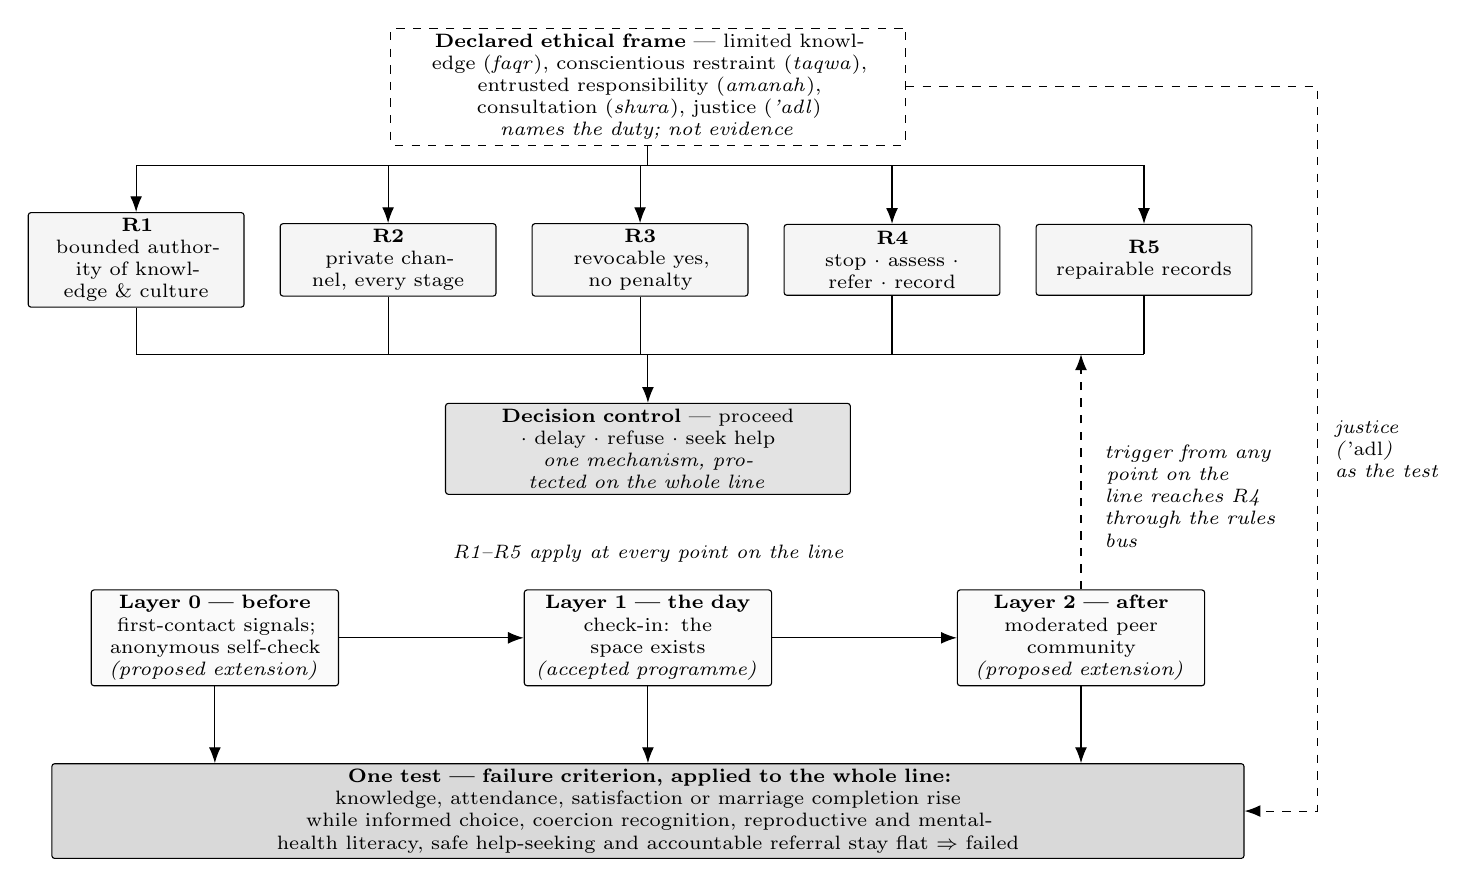
\begin{tikzpicture}[x=1mm,y=1mm,>={Latex[length=2mm]},
  box/.style={draw,rounded corners=1pt,fill=gray!8,align=center,font=\scriptsize,inner sep=2pt,minimum height=9mm},
  rule/.style={box,text width=26mm},
  layer/.style={box,text width=30mm,fill=gray!4},
  mech/.style={box,text width=50mm,fill=gray!22,minimum height=10mm},
  ethic/.style={box,text width=64mm,dashed,fill=white},
  test/.style={box,text width=150mm,fill=gray!30,minimum height=11mm},
  lab/.style={font=\scriptsize\itshape,align=left}]
\node[ethic] (E) at (85,100) {\textbf{Declared ethical frame} — limited knowledge (\emph{faqr}), conscientious restraint (\emph{taqwa}),\\ entrusted responsibility (\emph{amanah}), consultation (\emph{shura}), justice (\emph{\textquoteright adl})\\ \emph{names the duty; not evidence}};
\node[rule] (R1) at (20,78) {\textbf{R1}\\bounded authority of knowledge \& culture};
\node[rule] (R2) at (52,78) {\textbf{R2}\\private channel, every stage};
\node[rule] (R3) at (84,78) {\textbf{R3}\\revocable yes, no penalty};
\node[rule] (R4) at (116,78) {\textbf{R4}\\stop $\cdot$ assess $\cdot$ refer $\cdot$ record};
\node[rule] (R5) at (148,78) {\textbf{R5}\\repairable records};
\node[mech] (M) at (85,54) {\textbf{Decision control} — proceed $\cdot$ delay $\cdot$ refuse $\cdot$ seek help\\ \emph{one mechanism, protected on the whole line}};
\node[layer] (L0) at (30,30) {\textbf{Layer 0 — before}\\first-contact signals; anonymous self-check\\ \emph{(proposed extension)}};
\node[layer] (L1) at (85,30) {\textbf{Layer 1 — the day}\\check-in: the space exists\\ \emph{(accepted programme)}};
\node[layer] (L2) at (140,30) {\textbf{Layer 2 — after}\\moderated peer community\\ \emph{(proposed extension)}};
\node[test] (T) at (85,8) {\textbf{One test — failure criterion, applied to the whole line:} knowledge, attendance, satisfaction or marriage completion rise\\ while informed choice, coercion recognition, reproductive and mental-health literacy, safe help-seeking and accountable referral stay flat $\Rightarrow$ failed};
\draw (E.south) -- (85,90);
\draw (20,90) -- (148,90);
\foreach \r in {R1,R2,R3,R4,R5} \draw[->] (\r.north |- 0,90) -- (\r.north);
\foreach \r in {R1,R2,R3,R4,R5} \draw (\r.south) -- (\r.south |- 0,66);
\draw (20,66) -- (148,66);
\draw[->] (85,66) -- (M.north);
\draw[->] (L0.east) -- (L1.west); \draw[->] (L1.east) -- (L2.west);
\node[lab,anchor=north] at (85,43) {R1--R5 apply at every point on the line};
\foreach \l in {L0,L1,L2} \draw[->] (\l.south) -- (\l.south |- T.north);
\draw[->,dashed] (L2.north) -- (140,66);
\node[lab,anchor=west,text width=23mm] at (142,48) {trigger from any point on the line reaches R4 through the rules bus};
\draw[->,dashed] (E.east) -- (170,100) -- (170,8) -- (T.east);
\node[lab,anchor=west] at (171,54) {justice\\ (\emph{\textquoteright adl})\\ as the test};
\end{tikzpicture}}
\caption{Programme-theory diagram of \tphe{}, not a measured causal graph: no arrow represents an estimated effect. The declared ethical frame names the duty behind each rule; it is not evidence. Five rules (R1--R5) protect the single proposed mechanism, decision control; they apply at every point on one continuous timeline, of which only Layer 1 (the day) belongs to the accepted programme --- Layers 0 and 2 are extensions proposed for co-design. One pre-specified test is applied to the whole line; a trigger from any point on the line can invoke R4 (stop--assess--refer--record) directly, and justice (\emph{\textquoteright adl}) is the standard the failure criterion itself is tested against.}
\label{fig:dag}
\end{figure*}


\subsection{Definition and scope}
\textbf{Trustworthy Premarital Health Education (\tphe)} is a proposed governance architecture for
premarital education that aims to increase each participant's control over marriage-related health
decisions through five rules, a stop--assess--refer--record pathway, repairable documentation, and
prospectively testable outcomes. \emph{Trustworthy} names a condition the programme must earn through
observable practice; \emph{premarital} names the transition point, not one legal or religious form;
\emph{health education} spans physical, psychological, sexual and reproductive, relational,
legal-protection, and help-seeking literacy without turning educators into clinicians, lawyers,
investigators, or religious adjudicators; \emph{infrastructure} means repeatable roles, boundaries,
records, referral relationships, training, and accountability. \tphe{} is placed upstream, but when it
encounters existing violence or coercion its function changes to identification and safe routing; it
connects to competent secondary and tertiary responses without providing them.

\tphe{} is \emph{not}: a diagnostic instrument; a substitute for clinical, social, legal, emergency, or
survivor-advocacy services; couple therapy or reconciliation counselling; a promise to prevent
violence; a requirement that any participant leave or proceed; a universal Islamic ruling or a
culturally neutral model; evidence that any organisation's programme is effective; an autonomous AI
counselling system; or a checklist detached from training, referral capacity, and governance.

\textbf{From six safeguards to five rules.} The accepted abstract names six safeguards that protect
decision control: epistemic humility, cultural intelligibility, affected-person visibility, dignity
and consent, bounded authority and referral, and repairability. Below, these are operationalised as
five rules, R1--R5 (Table~\ref{tab:rules}), because epistemic humility and cultural intelligibility
answer the same audit question --- whose authority is this claim carrying, and where does that
authority end --- and are therefore implemented together as R1 (bounded authority of knowledge and
culture). Affected-person visibility maps to R2; dignity and consent to R3; bounded authority and
referral splits across R1 and R4; repairability maps to R5. Every safeguard named in the accepted
abstract survives this operationalisation; the change from six to five is a regrouping of duties into
auditable rules, not a retraction of any safeguard, and the same mapping applies wherever the two
vocabularies (``six safeguards'' and ``five rules'') appear elsewhere in this paper.

\subsection{The model as a continuous line}
The programme theory does not treat the classroom day as the intervention. It treats the whole
trajectory from first contact through the day of check-in to whatever follows as one governed line,
on which the mechanism, five rules, and one test apply throughout. Three layers mark points on that
line; only the middle layer, the day itself, is part of the accepted programme.

\subsubsection*{Layer 0 --- signals from first contact (proposed extension)}
Before enrolment, course-facing material can state plainly what fear, control, pressure, or unsafe
participation look like, that pausing or refusing is a normal outcome, and where private help is
available. An anonymous scored self-check --- a form, activity, or game, usable at any point on the
line --- lets a person see their own result and routes without submitting a name or a narrative unless
they choose to. No identity is required to complete it, and nothing is sent onward unless the person
acts on it. The nearest evidence family is decision-aid research, not a self-check validated for this
population: a Cochrane review of 209 decision-aid trials found consistent gains in knowledge and
values-congruent choice \cite{ref14}, while the closest content-matched online self-efficacy tool for
women experiencing abuse, I-DECIDE, found \emph{no} improvement in self-efficacy at 6 or 12 months in a
randomised controlled trial \cite{ref119,ref120}. That null result is reported here, not
set aside, because it is the closest outcome-domain precedent this proposed layer has. Because
access to a shared or partner-monitored device is itself a disclosure risk independent of what is
entered, any pilot implementation must leave no discoverable trace on a shared device (no login, no
tool-specific browser or app history, a quick-exit function) and must state this limitation to
users rather than implying anonymity of content is sufficient.

\subsubsection*{Layer 1 --- the day as check-in}
The day of delivery is reframed as a check-in at which a participant verifies in person whether the
declared protections are in place: a private slot the partner cannot see or control, a professional
interpreter rather than a family member, and an assessor with no stake in whether the wedding
proceeds. Attendance on this day evidences that the space exists; it evidences nothing about whether
the programme changed anyone's decisions, knowledge, or safety. Five rules govern conduct on the whole
line and are auditable at any point, not only on the day. Table~\ref{tab:rules} states each rule's
duty, one observable trace, and one falsifier.

\begin{table*}[t]
\centering\footnotesize
\caption{The five rules (R1--R5), one observable trace and one falsifier each. Programme theory;
none of these traces has yet been measured against an outcome.}
\label{tab:rules}
\begin{tabularx}{\textwidth}{@{}p{0.9cm}YYY@{}}
\toprule
& \textbf{Duty} & \textbf{Observable trace} & \textbf{Falsifier}\\
\midrule
R1 & Bounded authority of knowledge and culture: state what is known, uncertain, or needs qualified
advice; culture or religion never closes a safety or consent question. & Uncertainty and role
boundaries stated in audited sessions; referral for out-of-scope questions. & A session in which a
cultural or religious claim is used to end a safety or consent question rather than to refer it.\\
R2 & A private channel for every person, at every stage, that the partner cannot see or control;
interpretation is provided by a trained, confidentiality-bound professional interpreter with
no prior relationship with either participant's family, never by a family member. & A routinely offered, safely designed private slot; uptake logged
without content. & A person who wanted a private slot did not receive one, or a family member
interpreted a safety-relevant exchange.\\
R3 & Revocable yes: pause, delay, refusal, or non-completion is a normal outcome, without penalty, at
any point on the line. & A pause, delay, or refusal recorded without an accompanying penalty or
exclusion. & A participant who paused, delayed, or refused was excluded, penalised, or pressured to
reverse the decision.\\
R4 & Stop--assess--refer--record: a trigger from any point on the line (self-check, private slot,
peer community, direct observation) stops joint work, moves to private assessment by a qualified,
competence-bounded assessor, refers to a qualified multidisciplinary service such as Thailand's
One-Stop Crisis Centre (OSCC) or an equivalent designated service, counts referral at connection, and
records the sequence; joint work does not resume where coercive control is confirmed. No couple
mediation continues once coercive control is confirmed. \emph{Proposed extension, not yet
accepted:} that assessor should additionally
have no stake in whether the wedding proceeds and no prior personal, family or congregational
relationship with either participant that a reasonable observer would see as compromising
independence, drawn where possible from outside the couple's own community network (analogy
evidence only; \cite{ref158,ref159,ref162,ref163}). If a qualified assessor cannot be reached
within a pre-specified maximum interval, or assessment is inconclusive, the default is continued
stop, not resumption; the case is escalated to a named safeguarding lead, not closed by facilitator
judgement. & Time from trigger to a qualified private assessment; referral
offered, connected, and recorded. & Joint work continued, or resumed, after a trigger without
a documented safe assessment; a case resumed or closed by facilitator judgement because an assessor
was unavailable, without safeguarding-lead sign-off.\\
R5 & Repairable records: every entry has a named owner, a review date, and is corrected when new
information arrives. & A review completed on or before its scheduled date, with a dated correction
where warranted. & A record that is never reviewed, or a correction that overwrites the original
entry rather than appending to it.\\
\bottomrule
\end{tabularx}
\end{table*}

If danger appears imminent, the routine R4 sequence is suspended in favour of the organisation's
emergency protocol: immediate safety planning and contact with emergency services or the OSCC
emergency line take precedence over scheduling confidential assessment. Facilitators are trained to
recognise the difference and are never the final decision-maker for either pathway. A named
safeguarding lead, independent of routine facilitation duty, owns supervision, escalation decisions
and incident review; the assessor judges the individual case, and the safeguarding lead owns the
system.

\subsubsection*{Layer 2 --- moderated peer community after the course (proposed extension)}
After delivery, a moderated peer space, anonymous by choice, is proposed as a route through which the
same rules keep operating rather than as a service in its own right: a place to keep the self-check
and the private channel alive, with a moderator trained to route a real trigger to R4 and never to
mediate. It carries no promise of support beyond that routing function. The nearest evidence families
are online peer-support research, where moderation quality is repeatedly identified in realist syntheses
as the factor that determines whether a space helps or harms \cite{ref140,ref144}, with mixed
effectiveness reported for youth mental-health peer forums specifically \cite{ref139}, and
technology-facilitated-abuse
research, which documents how an unmoderated or poorly bounded digital channel can itself become a
vector for surveillance, harassment, or coercive control \cite{ref149,ref150}. Neither literature was
generated on a Muslim or Thai premarital population, and the pairing is by analogy, not by direct
evidence for this layer. A pilot of Layer 2 requires, at minimum, technically enforced anonymity (no
real names, no shared-device login trace), a moderator-independent one-tap report channel that
routes directly to R4, and a periodic anonymous safety poll of members; none of this exists yet, and
Layer 2 should not be piloted without it.

\subsubsection*{One test over the whole line}
The programme theory has a single, pre-specified failure criterion, applied to the mechanism, the
rules, and every layer together rather than to any one point on it. Stated verbatim from the accepted
abstract: \tphe{} fails if it raises knowledge scores, attendance, satisfaction, or marriage completion
while leaving informed choice, recognition of coercion, reproductive and mental-health literacy, safe
help-seeking, and accountable referral unchanged. A polished, well-attended programme that leaves
those outcome domains flat has failed as public-health infrastructure, whatever its conventional
metrics show.

\subsection{The declared ethical frame}
The programme's own ethical language is named here as a declared frame, not as evidence: it states the
duty an actor is held to, while the evidence in Table~\ref{tab:rules} and elsewhere states what is
known about the corresponding construct. The two are never substituted for one another.
\emph{Faqr} (acknowledging one's own incompleteness and dependence) governs the humility required by
R1. \emph{Taqwa} (conscientious restraint in the use of knowledge and power) governs the same
boundary in R1 together with the stop obligation in R4. \emph{Amanah} (authority and knowledge held as
an entrusted responsibility, to be returned to whom it belongs) governs the private channel of R2, the
revocable consent of R3, and the repairable records of R5. \emph{Shura} (consultation when a limit is
reached) governs the assessor and referral step within R4. \emph{'Adl} (justice, tested by whether the
less powerful person keeps dignity, rights, voice, and a route to repair) is the standard the
failure criterion applies. Table~\ref{tab:ethic} pairs each term with the rule it governs, the
evidence category that speaks to the underlying construct, distinct from the term itself, and an
evidence tier (external evidence, analogy, open, or practitioner-derived) so a reader can see how
directly each pairing is supported. None of the humility- or compassion-adjacent literature cited below
was generated on a Muslim or Thai sample; it is adjacent-population evidence, not evidence for this
population.

\begin{table*}[t]
\centering\footnotesize
\caption{The declared ethical frame: term, gloss, governed rule, evidence category paired with it, and
the evidence tier. The term names a duty; the evidence category speaks to the construct, not to the
term. External-evidence and analogy citations are from adjacent, non-Thai, non-Muslim, non-premarital
populations unless stated otherwise. R4's no-stake-assessor clause, governed here by \emph{Shura},
is a proposed extension, not yet part of the accepted programme (Table~\ref{tab:rules}).}
\label{tab:ethic}
\begin{tabularx}{\textwidth}{@{}p{1.4cm}YYYp{1.7cm}@{}}
\toprule
\textbf{Term} & \textbf{Plain-language gloss} & \textbf{Governs} & \textbf{Evidence category paired with it} & \textbf{Evidence tier}\\
\midrule
Faqr & Acknowledging one's own incompleteness and dependence. & R1 & Intellectual and relational
humility, self-compassion \cite{ref209,ref211,ref212,ref213}; declared-frame companion literature in
Islamic medical ethics \cite{ref226,ref228}. & External evidence (analogy); no Muslim or Thai samples
for the humility\slash compassion constructs.\\
Taqwa & Conscientious restraint in the use of knowledge, speech, judgement, and power. & R1, R4 &
Self-regulation and provider-boundary and referral literature. & Open: no evidence pairing identified
for this construct at this population.\\
Amanah & Authority and knowledge held as an entrusted responsibility, returned to whom it belongs. &
R2, R3, R5 & Consent, autonomy, and accountability literature. & Open: no evidence pairing identified
for this construct at this population.\\
Shura & Consultation when a limit is reached. & R4 (assessor and referral step) & Independent-advocate
and dual-relationship literature \cite{ref158,ref159,ref162,ref163}. & Analogy: transplant-advocate and
dual-relationship ethics, not domain-matched.\\
'Adl & Justice: whether the less powerful person keeps dignity, rights, voice, and a route to
repair. & The failure criterion & Outcome-domain and safeguarding literature the failure criterion is
built from (see discussion \S4.3). & Practitioner-derived: the criterion itself is authored for this
paper, not drawn from a single cited instrument.\\
\bottomrule
\end{tabularx}
\end{table*}

\subsection{Labelling: what is accepted and what is proposed}
The mechanism, the five rules, the stop rule, and the failure criterion restate the accepted abstract
and carry its claim ceiling: no effectiveness claim is made anywhere in this line. \textbf{Layer 0
(signals from first contact and the anonymous self-check), Layer 2 (the moderated peer community), and
the no-stake assessor are extensions proposed for co-design after the abstract's acceptance.} They are
not part of the accepted programme theory, they add no outcome claim of their own, and any public text
using them must say so explicitly. Where the evidence base for a proposed extension is open in either
direction, that status is stated plainly rather than framed as a mild or roughly neutral uncertainty.

\subsection{Testable propositions}
Table~\ref{tab:props} converts the framework into a research agenda capable of producing disconfirming
evidence. These are propositions for prospective testing, not results.

\begin{table*}[t]
\centering\footnotesize
\caption{Testable propositions, competing explanations, and evidence that would weaken or falsify each.}
\label{tab:props}
\begin{tabularx}{\textwidth}{@{}p{0.6cm}YYY@{}}
\toprule
& \textbf{Proposition} & \textbf{Competing explanation} & \textbf{Weakening / falsifying evidence}\\
\midrule
P1 & A governance layer improves decision control beyond content-only education & Knowledge or
facilitator warmth explains any gain & No added gain in decision control after controlling for
knowledge and facilitator effects\\
P2 & A routine private channel makes materially relevant concerns more visible & Private contact adds
burden without information & No increase in safe voice or appropriate routing, with more distress,
retaliation, or privacy risk\\
P3 & R1's cultural-intelligibility component improves comprehension and trust only when culture or
religion cannot override consent or safety & Cultural tailoring alone suffices & Tailoring improves
satisfaction but leaves consent pressure or unsafe authority unchanged\\
P4 & A stop rule prevents routine joint education from worsening risk when fear or coercion appears &
Skilled facilitators can manage all concerns jointly & The stop rule causes more net harm than
governed alternatives, or does not reduce unsafe joint exposure\\
P5 & Referral quality depends on timeliness, accessibility, and follow-through, not offer alone &
Information is enough & Connection and safety do not vary by latency, accessibility, or
follow-through\\
P6 & Conventional programme success can coexist with \tphe{} failure & Conventional outcomes
represent benefit & Conventional outcomes reliably predict decision control, help-seeking, and
referral fidelity\\
P7 & R5 (repairable records) is necessary because relevant information emerges over time & One-time
assessment suffices & Review and correction add no safety or accuracy benefit and introduce more harm
or burden\\
\bottomrule
\end{tabularx}
\end{table*}


\subsection{Research and development pathway}
Phase~0: framework clarification and evidence mapping (definitions; alignment with WHO RESPECT and clinical guidance and Thai service pathways; inventory of validated brief screens and measures; legal and data-governance review; distinguishing current ARAYA practice from proposed pilot requirements; external advisory group with conflict-of-interest management). Phase~1: co-design and content validation with survivors and advocates, Muslim and intercultural community members, Thai and non-Thai prospective participants, obstetric, reproductive-health, mental-health, social-work, substance-use, legal, and crisis-service professionals, Health Region~12, provincial Islamic committees, educators, interpreters, and data-governance expertise. Phase~1 is expected to proceed through facilitated co-design workshops together with cognitive interviewing of draft outcome instruments, with an indicative participant range of approximately 4--8 per stakeholder group, stated here as indicative rather than fixed. It would be chaired by an independent chair from outside ARAYA Nikah, and any activity involving survivors or community members would be sought through an accredited Thai research-ethics committee (for example a Health Region~12 provincial-hospital REC or an independent REC) before it begins. Phase~2: feasibility and safety pilot with pre-specified progression criteria---testing whether \tphe{} can be delivered safely and consistently, not whether it reduces violence. Phase~3: prospective comparative evaluation with decision control as primary candidate outcome, provided equipoise, safety, and referral standards are protected in all arms; violence reduction is not claimed without adequate power, follow-up, and attention to disclosure bias. The failure criterion and primary outcome set will be deposited in a public registry (for example the Thai Clinical Trials Registry) before Phase 3 data collection begins. Phase~4: independent replication outside ARAYA and in different legal, service, religious, and cultural settings.

\section{Discussion}

\subsection{Principal findings}
\tphe{} shifts the organising question of premarital education from content delivery to the governance of choice. Values such as respect, consent, culture, and referral become trustworthy only when translated into roles, trigger criteria, private channels, competence boundaries, records, review points, and measurable outcomes.

\subsection{Novelty and standpoint}

\tphe{} is not proposed into an empty field. Table~\ref{tab:novelty} places it alongside six
adjacent bodies of practice and evidence already reviewed in \S4.3, stating only what each is
documented to do, measure, and not do, and what \tphe{} adds on top of it. The comparison is not a
claim that \tphe{} outperforms any row; no effectiveness evidence exists for \tphe{} itself.

\begin{table*}[t]
\centering\footnotesize
\caption{What existing frameworks and programmes do, measure, and do not do, against what \tphe{}
proposes to add. Descriptive only; several rows are not examined here at manual/curriculum level and
are marked accordingly. No effectiveness comparison is implied.}
\label{tab:novelty}
\begin{tabularx}{\textwidth}{@{}p{2.1cm}YYYY@{}}
\toprule
& \textbf{What it does} & \textbf{What it measures} & \textbf{What it does not do (as documented)} & \textbf{What \tphe{} adds}\\
\midrule
WHO RESPECT & Names seven population-level prevention strategies for violence against women, synthesised across a global review of reviews \cite{who_respect,ref30}. & Framework-level: which strategy types have supporting reviews, not a single programme's outcomes. & Only 6/178 reviews updating it targeted relationship-skills strengthening specifically \cite{ref30}; it does not specify a premarital governance layer, a stop rule, or an assessor with no stake in the outcome. & Places one governance layer, with a named mechanism and stop rule, inside RESPECT's relationship-skills strategy, at the marriage transition specifically.\\
\addlinespace
Thai premarital course, southern provinces / Health Region 12 & Delivers premarital content within the government health-region system in Thailand's southern border provinces. \emph{Not examined here at manual level.} & Not established by any PubMed-indexed record in this review; no Thai premarital-education outcome study was located. & Not examined here --- this paper does not state whether it has, or lacks, a stop-and-refer rule, because its manual has not been reviewed. & A published, auditable rule set (R1--R5) and failure criterion that any programme, including this one, can be checked against.\\
\addlinespace
Malaysian Islamic pre-marriage course (Kursus Pra-Perkahwinan Islam) & Reported, not independently verified by this review, to be administratively linked to marriage registration for Muslim couples in Malaysia; content analysed through a moral-education lens at one Kuala Lumpur centre \cite{charoenwong2025} (non-PubMed, context only). & Moral-education framing of curriculum content at one centre; not an outcome trial. & Not shown, in the cited source, to measure decision control, coercion recognition, or safe help-seeking. & A decision-control mechanism and stop rule layered onto administratively mandatory delivery, not assumed present in it.\\
\addlinespace
Relationship\slash marriage education (MRE, PREP) & Structured curricula teaching communication and conflict skills, evaluated across cumulative meta-analyses \cite{ref6,ref7,fawcett2010}. & Relationship quality, communication skill, and (more recently) mental health and coparenting; effects small ($d\approx0.03$--$0.45$) \cite{ref6,ref7}. & Does not measure informed choice, coercion recognition, or safe help-seeking; higher-conflict couples showed a harmful-moderation pattern in one 8-year RCT \cite{ref9}. & A stop rule that withholds joint communication/conflict training precisely where coercive control is suspected, rather than delivering it universally.\\
\addlinespace
IPV screening in health settings & Structured clinical inquiry about intimate-partner violence, reviewed in a Cochrane review and the 2025 USPSTF evidence report \cite{ref38,ref39,ref40}. & Identification (OR 2.95 for increased detection \cite{ref38}); instrument sensitivity 26--87\% \cite{ref39}. & No evidence of an effect on referral (OR 2.24, 2 studies) or re-exposure at 3--18 months \cite{ref38,ref39}; WHO guidance conditions inquiry on a functioning referral system already existing \cite{ref43,ref44}. & Referral counted at the point of connection, not at the point of offer, plus a record that is reviewed and corrected rather than closed at first entry.\\
\addlinespace
Digital safety decision aids (I-DECIDE, myPlan) & Scored, self-directed online tools that let a person assess risk and see safety options privately \cite{ref119,ref120,ref123,ref124}. & Self-efficacy, reproductive coercion, depressive symptoms; the largest RCT found no self-efficacy gain at 6 or 12 months \cite{ref120}. & Not built for, or tested at, the premarital transition; not linked to an in-person stop--assess--refer pathway. & An anonymous self-check offered as one entry point on a continuous line that also includes an in-person check-in and a named stop rule, not a standalone tool.\\
\addlinespace
Faith-integrated health interventions (mosque-based RCTs) & Structured health curricula delivered by imams or lay religious facilitators, tested in cluster-randomised trials \cite{ref231,ref232}. & Clinical and psychological outcomes: 12-month type 2 diabetes incidence (9.8\% vs 17.1\%, aHR 0.75) \cite{ref231}; PTSD, depression and well-being effect sizes \cite{ref232}. & Neither trial tests premarital content, decision control, or coercion recognition; delivery-channel precedent only. & Uses the same trusted-channel logic for premarital delivery, paired with a bounded-authority rule (R1) that keeps religious framing from closing a safety question.\\
\bottomrule
\end{tabularx}
\end{table*}

Read across the rows, \tphe{}'s claimed novelty is not a new curriculum topic; every topic in the
right-hand column already exists somewhere in the left-hand column. The novelty is a governance
layer placed around premarital education, with decision control --- each participant's ability to
proceed, delay, or refuse, and to seek help safely --- named as the mechanism, rather than
knowledge gain, attendance, satisfaction, or completion. Four design choices follow directly from
gaps documented above, not from this paper's own preference. First, a private channel for every
person at every stage answers the finding that screening increases identification without a shown
effect on referral or re-exposure \cite{ref38,ref39}: a channel that exists before, during, and
after the day is a different exposure than a single clinical question. Second, the stop rule --- joint
work suspended on any trigger, resumed only after private assessment by a no-stake assessor, and
never resumed where coercive control is confirmed --- follows from the couples-therapy literature's
own caution: the only systematic review of conjoint IPV treatment called it viable only in select
situations after screening 1{,}733 citations to 6 eligible studies \cite{ref45}, and clinical
literature treats distinguishing situational couple violence from coercive controlling violence as a
prerequisite for any joint work at all \cite{ref46,ref47}. Communication and conflict training,
which MRE/PREP delivers by default, is accordingly withheld rather than delivered wherever that
distinction cannot yet be made. Third, counting referral at connection, not at offer, follows from
the same screening literature showing identification without a demonstrated referral effect
\cite{ref38,ref41} and from an emergency-department programme in which most screened patients could
not recall receiving a resource guide despite high screening rates \cite{ref173}: identification
without response is not treated here as response. Fourth, repairable records and a pre-specified
failure criterion follow from the recurring knowledge-to-behaviour gap this review documents twice
over --- premarital screening and thalassaemia education produce knowledge gains without matching
uptake \cite{ref12,ref13}, and decision-aid research shows values-congruent choice can improve while
self-efficacy in the closest content-matched trial did not \cite{ref14,ref120} --- so \tphe{}
pre-declares that raising knowledge, attendance, satisfaction, or marriage completion while leaving
informed choice, coercion recognition, and safe help-seeking unchanged counts as failure, not
success. The extensions proposed for co-design --- signals from first contact, an anonymous
self-check, and a moderated peer community --- extend this same logic outward along the line rather
than adding new content, and carry the same evidence gaps stated where each is first defined
above.

\textbf{Standpoint.} This proposal is made from the standpoint of a social-enterprise practitioner
and citizen with a direct process position in the transaction it describes --- someone who sits
inside the premarital-education relationship, not above it, and who has run one such programme since
2024. It does not speak from clinical, scholarly, legal, or religious authority, and none is
claimed. Those disciplines are respected on their own terms, and every construct this paper borrows
from them is paired with their own evidence, tiered honestly, in \S4.3 and Table~\ref{tab:ethic}. The
organisation's conflict of interest is disclosed in full (Declarations). The failure criterion stated
above, not the author's or the organisation's own account of its programme, is the standard this
proposal asks to be judged by.

This comparison and standpoint are offered as the basis for the co-design invitation in Phase~1 of
the research and development pathway described above, not as a claim that \tphe{} works.


\subsection{Comparison with existing frameworks and literature}

\tphe{} is compared here against the literature it draws on and is answerable to, not against a
systematic review's full search strategy. Unless flagged otherwise, every citation below offers
adjacent, analogous, or precedent evidence for a construct \tphe{} uses --- never evidence that
\tphe{} itself, or any of its five rules, works. The full ten-topic narrative this synthesis
condenses, including the burden-of-disease case, the preconception-medicine analogue, the
peer-support and technology-facilitated-abuse literatures, the assessor-independence analogy,
decision-quality and digital self-assessment tool literature, language-access evidence, and the
tier-one Islamic bioethics companion literature, together with the evidence map for propositions
P1--P7 (Table~\ref{tab:evidencemap}), is reproduced in full, with every citation intact, in
Appendix~E (Extended evidence review).

\textbf{\tphe{} is proposed as an addition, not a replacement, to structures that already exist in
this region.} WHO's RESPECT framework already names relationship-skills strengthening as one of
seven population-level violence-prevention strategies, though a global review of reviews updating
it found only 6 of 178 eligible reviews targeted that strategy specifically \cite{who_respect,ref30}
--- a strategy named, not yet built out. Thailand's own Health Region~12 premarital course and
Malaysia's administratively mandatory Kursus Pra-Perkahwinan Islam, examined here only through a
moral-education content analysis at one Kuala Lumpur centre \cite{charoenwong2025}, show that a
premarital contact point can already be delivered at population scale in Muslim and Thai settings.
Neither is shown, in the sources available to this review, to carry a stop rule, a private channel
independent of the couple, or a pre-specified failure criterion. \tphe{} is offered as a governance
layer that could be added to structures such as these, not as a competing curriculum (full
comparison: Table~\ref{tab:novelty}, \S4.2).

\textbf{Knowledge gained at a premarital contact point does not reliably convert into the outcome
that contact point exists for.} Premarital genetic screening is the closest direct precedent:
premarital thalassaemia education raises knowledge ($p<0.001$) without reliably raising uptake
\cite{ref13}, and premarital sickle-cell-trait screening uptake across Africa pools under half of
eligible couples (47.82\%, 95\% CI 46.53--49.11), described as ``suboptimal'' \cite{ref12}. The
relationship-education literature shows the same dissociation at larger scale: across cumulative
meta-analyses, effects on relationship quality and communication skill are consistently small
($d\approx0.03$--$0.45$) \cite{ref6,ref7}; the most current synthesis of a government-funded
programme (Hawkins, 2022) found small effects on relationship quality ($d=0.114$) and skills
($d=0.132$) and non-significant effects on stability, parenting, and child well-being \cite{ref7};
and a meta-analysis of relationship aggression specifically (Karantzas, 2023) found $d\approx0.11$
overall, not statistically convincing when restricted to RCTs alone ($d\approx0.05$) \cite{ref8}.
None of this literature has measured informed choice, coercion recognition, or safe help-seeking.

\textbf{The same identification-without-response pattern motivates R4's referral-at-connection
rule.} A Cochrane review of 13 RCTs found IPV screening increased identification (OR 2.95) but no
evidence of an effect on referral (OR 2.24, 2 studies only) or on re-exposure at 3--18 months
\cite{ref38}. The 2025 USPSTF evidence report reviewed 35 studies ($n=18{,}358$): 3 RCTs
($n=3{,}759$) comparing screening with no screening found no significant reduction in IPV or other
outcomes over 3--18 months \cite{ref39}, and the companion 2025 recommendation statement retained
only a moderate-net-benefit judgement for reproductive-age women \cite{ref40}. Screening finds; it
does not, by itself, connect.

\textbf{Recognition and behaviour dissociate in the literature closest to Layer~0's premise.} The
strongest cautionary evidence for a proposed extension built around raising recognition is a 1-year
cluster RCT of Coaching Boys Into Men (16 high schools, $n=1{,}513$ male athletes): perpetration
fell, but recognition of abusive behaviours did not change (95\% CI $-0.15$ to $0.09$), and
bystander intentions were unchanged \cite{ref190} --- recognition and behaviour separating exactly
as \tphe{}'s failure criterion is built to catch. Layer~0's proposed anonymous self-check has a
direct, cautionary precedent of its own: I-DECIDE, a masked two-arm RCT ($n=422$, 79--80\% 12-month
retention), found no improvement in self-efficacy at 6 or 12 months, with scores slightly lower in
the intervention arm than control (mean difference 1.3, 95\% CI 0.3--2.3 at 6 months) and no
between-group difference in depressive symptoms \cite{ref119,ref120}. That null result
is reported here, not set aside, because it is the closest outcome-domain precedent this proposed
extension has.

\textbf{The stop rule's own evidence base is small and explicitly cautious.} The only systematic
review of couples therapy as an IPV treatment, after screening 1{,}733 citations, found only 6
studies met inclusion; pooled data suggested conjoint treatment ``viable in select situations,''
with professionals cautious about violent-retaliation risk \cite{ref45}. Survivor-voiced evidence
complicates any default toward joint response: only 9 of 17 women in one qualitative sample rated
couples counselling a good idea \cite{ref48}. This literature supports withholding routine joint
work where coercive control is confirmed; it does not demonstrate that any stop rule, including
\tphe{}'s, improves outcomes.

\textbf{Cultural-competence training repeatedly raises provider-level knowledge or attitudes without
a corresponding patient-outcome gain} --- the pattern R1's cultural-intelligibility safeguard is
built to answer, not to assume already solved. A Cochrane review of 5 RCTs (337 professionals,
8{,}400 patients) rated the evidence low-quality, with some improvement in involvement or
understanding but no reliable clinical-outcome effect \cite{ref55}; a narrower review found no
significant patient-outcome improvement in any of the studies it identified \cite{ref56}; and
Indigenous cultural-safety training across four high-income countries found outcomes overwhelmingly
provider-level, with weak clinical-outcome evidence \cite{ref57}.

\textbf{Religiosity is not a uniform protective factor, which is why the ethical frame (\S3.3) is
presented as a declared duty rather than as evidence.} A 67-study systematic review and
meta-analysis found religiosity and spirituality protective for general interpersonal aggression but
\emph{not} specifically for domestic violence \cite{ref220}, complicating any simple ``faith
protects'' reading and reinforcing why Table~\ref{tab:ethic} pairs each ethical term with a
separately evidenced construct rather than treating the term itself as a finding.

\textbf{Direct Thai evidence remains sparse and geographically uneven, and none of it evaluates a
premarital programme.} A four-region national survey ($n=2{,}462$ married or cohabiting women) found
roughly 15\% lifetime psychological, physical, or sexual IPV \cite{ref72}; among 700 Muslim
adolescents on the southern border, 9\% were sexually experienced, with condom non-use, STI, and
repeat pregnancy concentrated in that subgroup \cite{ref76}; and among 360 Muslim army conscripts in
the three deep southern provinces, 78.7\% showed poor HIV/STI-transmission knowledge \cite{ref77}.
No study identified in this review evaluates a premarital-education programme, of any design, with a
Thai Muslim or Thai intercultural population.

\textbf{Read together, this literature does two things and stops short of a third.} It makes a
premarital contact point plausible to build and deliver at population scale (preconception medicine,
premarital genetic screening, and Thailand's and Malaysia's own existing courses); it repeatedly
shows that knowledge, attendance, satisfaction, and provider-level attitude gains do not reliably
convert into the behavioural, referral, or patient-outcome change a programme is built to produce
(screening, relationship education, and cultural-competence training alike). It does not show that
any premarital governance layer, of this or any design, changes informed choice, coercion
recognition, or safe help-seeking --- because no such test has yet been run. \tphe{} is offered as a
falsifiable synthesis awaiting that test, never as evidence that premarital education of this design
improves, prevents, or reduces any outcome. The full evidence base this synthesis draws from,
organised by proposition (P1--P7) and by topic, is in Appendix~E.


\subsection{Ethical root: faqr, taqwa, amanah, and justice}\label{sec:root}
The framework does not treat culture as a barrier to be removed. Its epistemic-humility safeguard rests on a working sequence: \emph{faqr} makes us aware of our own incompleteness and dependence on God (Qur'an 35:15); \emph{taqwa} is God-conscious restraint over one's knowledge, speech, judgement, and use of power (Qur'an 59:18); \emph{amanah} frames authority and knowledge as an entrusted responsibility to be rendered to those to whom it belongs, placed by the Qur'an beside just judgement (4:58). \emph{Faqr}'s classical sense is existential neediness before God; this paper narrows it to the epistemic case (what one does not know) as one instance of that neediness, not as a redefinition of the term. \emph{Shura} is the method of acting when limits are reached (42:38); it accompanies the sequence and does not replace \emph{taqwa} within it. \emph{'Adl} is the test: not whether the person holding authority meant well, but whether the affected person retains dignity, rights, voice, and a real route to correction.

Applied to the family, in the author's formulation: \emph{faqr} makes us aware of our own incompleteness and our dependence on God; because no one is complete, the members of a family must depend on and be responsible to one another, with \emph{taqwa} as the governing restraint, and with \emph{amanah} made visible through the steady, dependable fulfilment of duties that never violate one another's rights. Mutual dependence is the reason a family needs safeguards; \emph{taqwa} is why authority within it must be restrained; \emph{amanah} is why fulfilling one's role and respecting the other's rights are the same act rather than competing ones. Humility here is not passivity: a person may fulfil duties, ask for help, challenge misuse of authority, and claim rights with humility, and a teacher who admits uncertainty must still act when safety procedures require it. This is compatible with cultural humility in health education \cite{ref58}. The sequence is this paper's conceptual synthesis; the terms are Qur'anic, the architecture is not a model declared by the sources, and full jurisprudential interpretation requires qualified scholarship. Where Table~\ref{tab:ethic} marks a term's evidence pairing Open, the rule it governs (R1 for taqwa, R2/R3/R5 for amanah) is supported only by the rule's own falsifier and observable trace in Table~\ref{tab:rules}, not by external evidence for the ethical term itself.

\subsection{Implications for practice and policy}
Without a failure criterion, programmes can absorb safeguarding language while retaining continuation-oriented incentives. If knowledge and satisfaction rise while a person remains unable to pause, refuse, recognise coercion, or reach qualified help, the mechanism has not been achieved. Infrastructure should be judged by what it enables under pressure, not by what it teaches under ideal conditions. A scenario simulation over declared assumptions (Appendix~F) ranked pre-arranged assessor, room and interpreter, a facilitator-training gate, a narrow trained trigger list and a follow-up slot as the delivery conditions most likely to decide whether the stop rule can be executed; it produces no evidence about outcomes.

\subsection{Institutional position}
Why does a social enterprise, rather than a clinical, academic, or religious institution, convene this synthesis? What follows is a declared position, not an evidentiary claim, and it rests on process, not authority. ARAYA Nikah occupies what this paper calls the process position: it is present with a couple across the weeks before a wedding, controls the sequence in which content, documentation, and referral are offered, and observes what actually happens at the point where consent, authority, and help-seeking are organised. That sustained proximity is not ordinarily available to a single clinic visit, a one-off curriculum audit, or a legal review conducted after the fact.

The organisation is registered, per the organisation's own governance records, under Thailand's Social Enterprise Promotion Act B.E.~2562, which binds it in law to a declared social objective and limits the distribution of profit. That legal binding, and no broader legal claim, is what is asserted here; the Act's other provisions, and any claim about prenuptial law or domestic-violence law reform, are outside this paper's competence and are not made. Because the organisation's continuation does not depend on completing marriages, it can afford to declare a failure criterion that treats marriage completion as irrelevant to success --- a criterion a fee-for-service or completion-incentivised provider would find harder to state without undermining its own model.

This position carries no authority of its own, and none is claimed. It offers depth in one relationship, repeated many times, not population coverage; a clinical, academic, or religious body with broader reach and different obligations is not replaced by it and is not asked to defer to it. Its legitimacy is borrowed, not earned: it stands until survivors, advocates, religious and community leaders, and independent reviewers examine the procedures described in this paper and say plainly whether they hold up. Being bound by law to a social objective changes what the organisation's incentives are re-bound to; it does not remove incentive, interest, or the founder's disclosed conflict (Declarations), and none of the above is offered as a substitute for that independent review.

\subsection{Implications for research: transferability and next steps}
\tphe{} originated in a Muslim-led Thai practice environment but addresses a general problem. Transferability is an empirical question. Adaptation may change language, examples, religious sources, legal procedures, service partners, facilitators, and settings; it must preserve the invariants: the participant, not marriage completion, is the unit of protection; usable decision control is the mechanism; each person has a safe private route; culture and religion do not override consent or safety; educator authority is bounded; fear, violence, or coercive control changes the course of education; qualified referral takes priority beyond competence; decisions and records can be reviewed and corrected; conventional outcomes cannot substitute for safeguarding outcomes.

\subsection{Artificial intelligence: boundary only}
AI is not part of the \tphe{} mechanism and is not an evaluated intervention (distinct from the manuscript-drafting disclosure in Declarations). Any future exploration is limited to facilitator-reviewed drafting of teaching materials or fictional scenarios, with no AI counselling, no autonomous safety decisions, no automated classification of violence or coercion, and human review for accuracy, cultural meaning, safety, and bias. No participant data are entered into any AI system; the anonymous self-check (Results, Layer~0), if used, is scored without AI.

\subsection{Strengths and limitations}
Strengths: the programme theory is stated with a pre-specified failure criterion, named outcome domains, and seven propositions with falsifiers, before any effectiveness testing; the claim ceiling is explicit; the conflict of interest is disclosed. Limitations: (1)~Derived from one founder-led organisation. (2)~Not a formal qualitative study: no systematic sampling, independent coding, or participant validation. (3)~No effectiveness or safety testing; the mechanism, safeguards, measures, and pathway may prove incomplete, burdensome, or harmful. (4)~Grounded in Muslim and intercultural couples in Thailand; not representative of all Muslim communities, Thai settings, or non-Muslim contexts. (5)~Identifies a governance problem without establishing that existing programmes lack comparable safeguards; direct claims about any programme require its complete procedures to be examined. (6)~Decision control is not a validated measure and may overlap with autonomy, self-efficacy, informed choice, safety, and service access. (7)~Referral capacity is context-dependent. (8)~Founder authorship creates conflict of interest; independent co-design, external review, and replication are necessary.

\subsection{Invitation to co-design}
This framework is offered at the point where practice-derived synthesis must stop and shared testing must begin. ARAYA Nikah does not propose to validate \tphe{} alone, and does not claim the authority to decide what ``trustworthy'' means for communities it does not represent. What the organisation can offer into a Phase~1 co-design process (\S3.6, ``Research and development pathway'') is what this paper has already made explicit and auditable: its governance and safeguarding procedures, its stop--assess--refer--record pathway, its documentation practice, its practice context of 600+ participants offered here as demand for this work, not evidence that it succeeds, and a pre-specified failure criterion against which its own work is willing to be judged --- \tphe{} fails if knowledge, attendance, or satisfaction rises while informed choice and accountable referral do not.

Co-design under that criterion needs partners this paper cannot substitute for. Survivors and advocates are needed to test whether the private channel and the stop rule protect rather than perform protection. Health Region~12 and its existing premarital services are needed as the clinical and public-health infrastructure this framework is designed to add governance to, not replace. Provincial Islamic committees are needed because premarital education in the deep South already has standing and reach this framework does not. This framework does not yet know, and does not assert, whether OSCC and equivalent referral services are reachable within a safe timeframe across all delivery sites, including after-hours and in Malay/Yawi-medium settings, or how a state referral pathway is meant to interact with a participant's existing recourse to family or religious dispute resolution; these are named here as open questions for Phase~1, not as solved problems. Referral services, including One-Stop Crisis Centres (OSCC) and other designated multidisciplinary services, are needed to confirm that the pathways named here are real, timely, and accessible where couples actually live. TIMA/FIMA members are needed as the clinical judgement this synthesis was never positioned to supply on its own.

Phase~1 would be chaired independently of ARAYA Nikah, with decision authority in a steering group on which the organisation holds one seat and no veto. Materials co-developed in Phase~1 would be held by the co-design consortium under a Creative Commons Attribution (CC~BY~4.0) licence, not by the company. Partners take on reputational exposure to a framework that has not yet been tested; the failure criterion and the right to withdraw at any phase are offered as the protection against that exposure.

The organisation's contribution ends where these partners' expertise begins. What is asked in return is not endorsement but scrutiny: a Phase~1 co-design process free to keep, revise, or reject any element of this synthesis, tested against the failure criterion stated above and in the accepted abstract. Nothing here proceeds to scale before feasibility and safety testing (Phase~2) confirm that \tphe{} can be delivered safely and consistently, before any claim of effectiveness is made.

\section{Conclusion}
Premarital health education is a consequential decision environment. When it teaches couples but cannot protect the individual participant, stop unsafe joint work, refer beyond educator competence, or correct an earlier decision, it remains incomplete as public-health infrastructure. \tphe{} proposes one mechanism---decision control---protected by six safeguards, operationalised as five rules (R1--R5), and a stop rule under which routine couple education yields to confidential assessment, survivor-centred support, and qualified referral. The framework is not yet validated; its value will depend on whether co-design and empirical testing show that it improves usable choice and accountable routing without creating new harms. Judge premarital health education not by how many marriages it completes, but by how safely people can choose. That judgement is not the organisation's to make alone: it is offered to TIMA/FIMA, Health Region~12, provincial Islamic committees, referral services, survivors, and advocates as an invitation to co-design and test this framework together, under the failure criterion stated above, before any claim of effectiveness is made.

\section*{Declarations}
\addcontentsline{toc}{section}{Declarations}
\footnotesize
\textbf{Conflict of interest.} The author is the founder and programme developer of ARAYA Nikah Social Enterprise Co., Ltd., the organisation whose procedures informed this synthesis, and has a reputational and commercial interest in the programme described. This conflict is disclosed in every public version of the work. No grant or award funded this work.\\
\textbf{Funding.} None.\\
\textbf{Ethics.} This conceptual paper involved no participant research, no participant data, and no identifiable information. Any co-design, cognitive interviewing, pilot data collection, or evaluation will undergo ethics review before it begins.\\
\textbf{Data availability.} No participant dataset was generated or analysed. The scenario-simulation code and its declared parameters (Appendix F) are available from the corresponding author on request.\\
\textbf{Use of AI.} AI tools assisted drafting and editing; the author verified all content and is accountable for it. No participant data are entered into any AI system; the anonymous self-check (Results, Layer~0), if used, is scored without AI.\\
\textbf{Author contributions.} YL conceived the framework, conducted the synthesis, and wrote the manuscript; there are no further contributors.\\
\textbf{Acknowledgements.} The author thanks the organisation's team for their support during the development of this work.\\
\textbf{Disclaimer.} This paper is a theoretical framework. It is not medical, legal, or religious advice, not a diagnostic instrument, and not a substitute for qualified clinical, legal, or survivor-support services. Laws governing health advice, safeguarding, data protection, and marriage vary by jurisdiction; institutional, educational, or public use requires legal and professional review.

\balance
\begin{thebibliography}{999}\footnotesize
\bibitem{ref1} GBD 2023 IPV and SVAC Collaborators. Disease burden attributable to intimate partner violence against females and sexual violence against children in 204 countries and territories, 1990-2023: a systematic analysis for the Global Burden of Disease Study 2023. Lancet (London, England). 2026. PMID: 41386261.
\bibitem{ref2} Sardinha L. Global, regional, and national prevalence estimates of physical or sexual, or both, intimate partner violence against women in 2018. Lancet (London, England). 2022. PMID: 35182472.
\bibitem{ref3} Kuswanto H. Prevalence of and factors associated with female child marriage in Indonesia. PLoS ONE. 2024. PMID: 38968277.
\bibitem{ref4} Rumble L. An empirical exploration of female child marriage determinants in Indonesia. BMC Public Health. 2018. PMID: 29587705.
\bibitem{ref5} Islam MK. Attitudes to and experiences of intimate partner violence among Rohingya women who married before eighteen years of age. Global Health Action. 2021. PMID: 34323166.
\bibitem{ref6} Hawkins AJ. Does marriage and relationship education work? A meta-analytic study. Journal of Consulting and Clinical Psychology. 2008. PMID: 18837590.
\bibitem{ref7} Hawkins AJ. How effective are ACF-funded couple relationship education programs? A meta-analytic study. Family Process. 2022. PMID: 35040124.
\bibitem{ref8} Karantzas Gery C. Do relationship education programs reduce relationship aggression? A meta-analytic study. Clinical Psychology Review. 2023. PMID: 37499317.
\bibitem{ref9} Markman HJ. A randomized clinical trial of the effectiveness of premarital intervention: moderators of divorce outcomes. Journal of Family Psychology. 2013. PMID: 23421844.
\bibitem{ref10} Williamson HC. Risk moderates the outcome of relationship education: a randomized controlled trial. Journal of Consulting and Clinical Psychology. 2015. PMID: 25664643.
\bibitem{ref11} Benedetto Chiara. FIGO Preconception Checklist: Preconception care for mother and baby. International Journal of Gynaecology and Obstetrics. 2024. PMID: 38426290.
\bibitem{ref12} Dilli Priscilla Peter. Update on the practice of premarital screening for sickle cell traits in Africa: a systematic review and meta-analysis. BMC Public Health. 2024. PMID: 38822327.
\bibitem{ref13} Anwar. Characteristics and Effectiveness of Premarital Thalassaemia Educational Interventions Worldwide: A scoping review. Sultan Qaboos University Medical Journal. 2025. PMCID: PMC12445309; not PubMed-indexed.
\bibitem{ref14} Stacey Dawn. Decision aids for people facing health treatment or screening decisions. Cochrane Database of Systematic Reviews. 2024. PMID: 38284415.
\bibitem{ref15} Elwyn G. A three-talk model for shared decision making: multistage consultation process. BMJ. 2017. PMID: 29109079.
\bibitem{ref16} Upadhyay Ushma D. Development and validation of a reproductive autonomy scale. Studies in Family Planning. 2014. PMID: 24615573.
\bibitem{ref17} McCauley Heather L. Psychometric properties and refinement of the Reproductive Coercion Scale. Contraception. 2017. PMID: 27639927.
\bibitem{ref18} Upadhyay Ushma D. Development and Validation of the Sexual and Reproductive Empowerment Scale for Adolescents and Young Adults. The Journal of Adolescent Health. 2021. PMID: 32690468.
\bibitem{ref19} Dagher Myriam. Adaptation and psychometric assessment of a sexual and reproductive empowerment scale in Arabic among refugee and non-refugee adolescent girls. BMC Medical Research Methodology. 2024. PMID: 39266993.
\bibitem{ref20} Alomair N. Factors influencing sexual and reproductive health of Muslim women: a systematic review. Reproductive Health. 2020. PMID: 32138744.
\bibitem{ref21} Spencer CN. Health effects associated with exposure to intimate partner violence against women and childhood sexual abuse: a burden of proof study. Nature Medicine. 2023. PMID: 38081957.
\bibitem{ref22} Oram S. The Lancet Psychiatry Commission on intimate partner violence and mental health: advancing mental health services, research, and policy. The Lancet Psychiatry. 2022. PMID: 35569504.
\bibitem{ref23} Bacchus LJ. Interventions that prevent or respond to intimate partner violence against women and violence against children: a systematic review. The Lancet Public Health. 2024. PMID: 38702097.
\bibitem{ref24} Abramsky T. Findings from the SASA! Study: a cluster randomized controlled trial to assess the impact of a community mobilization intervention to prevent violence against women and reduce HIV risk in Kampala, Uganda. BMC medicine. 2014. PMID: 25248996.
\bibitem{ref25} Abramsky T. Ecological pathways to prevention: How does the SASA! community mobilisation model work to prevent physical intimate partner violence against women? BMC public health. 2016. PMID: 27084116.
\bibitem{ref26} Dunkle K. Effective prevention of intimate partner violence through couples training: a randomised controlled trial of Indashyikirwa in Rwanda. BMJ global health. 2020. PMID: 33355268.
\bibitem{ref27} Shaw B. Shifting Norms in Faith Communities to Reduce Intimate Partner Violence: Results from a Cluster Randomized Controlled Trial in Nigeria. Journal of interpersonal violence. 2023. PMID: 37329160.
\bibitem{ref28} Chatterji S. Community activism as a strategy to reduce intimate partner violence (IPV) in rural Rwanda: Results of a community randomised trial. Journal of global health. 2020. PMID: 32257154.
\bibitem{ref29} Jeong J. Effectiveness of the Moments that Matter parenting programme on caregiving practices, family violence, mental health and early child development in Kenya: a cluster-randomised controlled trial. BMJ global health. 2026. PMID: 42556995.
\bibitem{ref30} Ullman C. Interventions to prevent violence against women and girls globally: a global systematic review of reviews to update the RESPECT women framework. BMJ Public Health. 2025. PMID: 40017928.
\bibitem{ref31} Falb KL. Adapting, Sustaining and Scaling Violence against Women and Children Prevention Interventions in Low- and Middle-Income Countries: A Scoping Review on the Use of Implementation Science. Trauma, violence \& abuse. 2026. PMID: 40462272.
\bibitem{ref32} Doe Patience Fakornam. Couple-based preconception care as a gender-responsive strategy for improving health and well-being: a systematic review. Reproductive Health. 2026. PMID: 42316254.
\bibitem{ref33} Hawkins AJ. Exploring programmatic moderators of the effectiveness of marriage and relationship education programs: a meta-analytic study. Behavior Therapy. 2012. PMID: 22304880.
\bibitem{ref34} Bahrami-Samani S. Comparing the effects of premarital booklet- and video-based educations on the reproductive health literacy of engaged couples. Health Science Reports. 2024. PMID: 39377020.
\bibitem{ref35} Ashrafi E. Evaluating the Impact of Reproductive and Sexual Health Education on Knowledge and Attitudes of Couples in Premarital Counseling Classes: A Quasi-Experimental Study. Health Science Reports. 2026. PMID: 41773204.
\bibitem{ref36} Spencer CM. Online relationship education programs improve individual and relationship functioning: A meta-analytic review. Journal of Marital and Family Therapy. 2021. PMID: 33502054.
\bibitem{ref37} Robles TF. Marital quality and health: a meta-analytic review. Psychological Bulletin. 2014. PMID: 23527470.
\bibitem{ref38} O'Doherty L. Screening women for intimate partner violence in healthcare settings. Cochrane Database of Systematic Reviews. 2015. PMID: 26200817.
\bibitem{ref39} Feltner Cynthia. Screening for Intimate Partner Violence and for Caregiver Abuse of Older or Vulnerable Adults: An Evidence Report and Systematic Review for the US Preventive Services Task Force. JAMA. 2025. PMID: 40553460.
\bibitem{ref40} US Preventive Services Task Force. Screening for Intimate Partner Violence and Caregiver Abuse of Older or Vulnerable Adults: US Preventive Services Task Force Recommendation Statement. JAMA. 2025. PMID: 40553450.
\bibitem{ref41} Kalra Naira. Training healthcare providers to respond to intimate partner violence against women. Cochrane Database of Systematic Reviews. 2021. PMID: 34057734.
\bibitem{ref42} Betron. Effectiveness of a clinic-based counselling intervention on risk of experiencing intimate partner violence and reproductive coercion: a matched-pair cluster-controlled trial in Ebonyi and Sokoto, Nigeria. BMJ Global Health. 2025. PMID: 41151831.
\bibitem{ref43} World Health Organization. Responding to intimate partner violence and sexual violence against women: WHO clinical and policy guidelines. Geneva: World Health Organization; 2013. ISBN 978 92 4 154859 5. Available from: https://iris.who.int/handle/10665/85240; not PubMed-indexed.
\bibitem{ref44} World Health Organization. Health care for women subjected to intimate partner violence or sexual violence: a clinical handbook. Geneva: World Health Organization; 2014. WHO reference WHO/RHR/14.26. Available from: https://iris.who.int/handle/10665/136101; not PubMed-indexed.
\bibitem{ref45} Karakurt. Couples Therapy for Intimate Partner Violence: A Systematic Review and Meta-Analysis. Journal of marital and family therapy. 2016. PMID: 27377617.
\bibitem{ref46} McCollum. Couples treatment for interpersonal violence: a review of outcome research literature and current clinical practices. Violence and victims. 2008. PMID: 18624089.
\bibitem{ref47} Schneider. From scared to repaired: using an attachment-based perspective to understand situational couple violence. Journal of marital and family therapy. 2014. PMID: 25039387.
\bibitem{ref48} Chang. Health care interventions for intimate partner violence: what women want. Women's health issues. 2005. PMID: 15661584.
\bibitem{ref49} Robertson. Women and men's use of coercive control in intimate partner violence. Violence and victims. 2011. PMID: 21780535.
\bibitem{ref50} Swan. Factor structures for aggression and victimization among women who used aggression against male partners. Violence against women. 2012. PMID: 23012348.
\bibitem{ref51} Evans. "Even 'Daily' is Not Enough": How Well Do We Measure Domestic Violence and Abuse?-A Think-Aloud Study of a Commonly Used Self-Report Scale. Violence and victims. 2016. PMID: 26645540.
\bibitem{ref52} Skivington K. A new framework for developing and evaluating complex interventions: update of Medical Research Council guidance. BMJ. 2021. PMID: 34593508.
\bibitem{ref53} Moore G. Adapting interventions to new contexts-the ADAPT guidance. BMJ. 2021. PMID: 34344699.
\bibitem{ref54} Moore GF. Process evaluation of complex interventions: Medical Research Council guidance. BMJ. 2015. PMID: 25791983.
\bibitem{ref55} Horvat L. Cultural competence education for health professionals. Cochrane Database of Systematic Reviews. 2014. PMID: 24793445.
\bibitem{ref56} Vella Elizabeth. Does cultural competence training for health professionals impact culturally and linguistically diverse patient outcomes? A systematic review of the literature. Nurse Education Today. 2022. PMID: 35964378.
\bibitem{ref57} Hardy Billie-Jo. Systematic review of Indigenous cultural safety training interventions for healthcare professionals in Australia, Canada, New Zealand and the United States. BMJ Open. 2023. PMID: 37793931.
\bibitem{ref58} Tervalon M. Cultural humility versus cultural competence: a critical distinction in defining physician training outcomes in multicultural education. Journal of Health Care for the Poor and Underserved. 1998. PMID: 10073197.
\bibitem{ref59} Bresnahan Mary. Culturally safe healthcare: changing the lens from provider control to patient agency. Journal of Communication in Healthcare. 2024. PMID: 38426444.
\bibitem{ref60} Cano-Ibáñez Naomi. Physician-Patient Language Discordance and Poor Health Outcomes: A Systematic Scoping Review. Frontiers in Public Health. 2021. PMID: 33816420.
\bibitem{ref61} Chu Janet N. Association between language discordance and unplanned hospital readmissions or emergency department revisits: a systematic review and meta-analysis. BMJ Quality \& Safety. 2024. PMID: 38160059.
\bibitem{ref62} Heath Morten. Interpreter services and effect on healthcare - a systematic review of the impact of different types of interpreters on patient outcome. Journal of Migration and Health. 2023. PMID: 36816444.
\bibitem{ref63} Lauridsen Iben Gad. A systematic review of whether the number of linguistic errors in medical interpretation is associated with the use of professional vs ad hoc interpreters. Archives of Public Health. 2024. PMID: 39696623.
\bibitem{ref64} Reaume M. Patient-Physician Language Concordance and Cardiovascular Outcomes Among Patients With Hypertension. JAMA Network Open. 2025. PMID: 39969882.
\bibitem{ref65} Kosiyaporn Hathairat. Strengthening the migrant-friendliness of Thai health services through interpretation and cultural mediation: a system analysis. Global Health Research and Policy. 2020. PMID: 33372646.
\bibitem{ref66} König Andrea. A Systematic Scoping Review on Migrant Health Coverage in Thailand. Tropical Medicine and Infectious Disease. 2022. PMID: 36006258.
\bibitem{ref67} Phanwichatkul Titaree. The perceptions and practices of Thai health professionals providing maternity care for migrant Burmese women: An ethnographic study. Women and Birth. 2022. PMID: 34272187.
\bibitem{ref68} Buathong Napakkawat. Exploring symptoms perception and barriers to medication adherence among Thai Muslim patients with non-communicable diseases in a rural community in southern Thailand: a mixed-methods study. BMJ Open. 2024. PMID: 39653570.
\bibitem{ref69} Lohmae Userow. Muslim mothers' experiences in taking care of children with open heart surgery: A qualitative study in Southern Thailand. Belitung Nursing Journal. 2025. PMID: 40256382.
\bibitem{ref70} Pérez-Sánchez María. Access of migrant women to sexual and reproductive health services: A systematic review. Midwifery. 2024. PMID: 39243595.
\bibitem{ref71} Weschasat Tassanapan. The edutainment program on knowledge, perception, and uptake of cervical cancer screening among Muslim women in Southern Thailand: a quasi experimental study. BMC Public Health. 2024. PMID: 38971727.
\bibitem{ref72} Chuemchit Montakarn. Prevalence of Intimate Partner Violence in Thailand. Journal of Family Violence. 2018. PMID: 29904232.
\bibitem{ref73} Thananowan Nanthana. Intimate partner violence and factors associated with sexually transmitted infections among Thai women attending gynecology clinics. International Journal of STD \& AIDS. 2021. PMID: 33308089.
\bibitem{ref74} Thananowan Nanthana. Intimate partner violence among pregnant Thai women. Violence Against Women. 2008. PMID: 18408170.
\bibitem{ref75} Thitiyanviroj Benjaporn. Perceptions of Screening Women for Intimate Partner Violence Among Health Care Providers in Thailand. Nursing for Women's Health. 2024. PMID: 39536796.
\bibitem{ref76} Hayee Fusiyah. Sexual risk behaviors and influencing factors among Muslim adolescents on southern border of Thailand. International Journal of Adolescent Medicine and Health. 2020. PMID: 32549162.
\bibitem{ref77} Singkun Awirut. Risk of HIV/STIs among Muslim army conscripts in the three deep southern provinces of Thailand. Health Promotion Perspectives. 2021. PMID: 35079589.
\bibitem{ref78} Singkun Awirut. Sexual knowledge based on Islamic values and sexual risk behaviors of HIV/STIs among Thai Muslim army conscripts: A cross-sectional study. Belitung Nursing Journal. 2022. PMID: 37554485.
\bibitem{ref79} Ford Kathleen. Mental health in a conflict area: Migration, economic stress and religiosity in the three southernmost provinces of Thailand. International Journal of Social Psychiatry. 2017. PMID: 28024446.
\bibitem{ref80} Ford Kathleen. Mental health among youth in a conflict area: a cross-sectional study of the effects of parental absence, social media, family support and religious practice on psychiatric symptoms in Thailand's southernmost provinces. Conflict and Health. 2026. PMID: 41540416.
\bibitem{ref81} Vapattanawong Patama. A cross-sectional study on factors influencing adolescent depression in the civil-conflict areas of Thailand. BMC Public Health. 2026. PMID: 41872869.
\bibitem{ref82} Ford Kathleen. Coming of age in a conflict area: Mental health, education, employment, migration and family formation in the southernmost provinces of Thailand. International Journal of Social Psychiatry. 2018. PMID: 29417854.
\bibitem{ref83} Sirithammaphan Uraiwan. Barriers to measles mumps rubella vaccine acceptance in the three southern border provinces of Thailand. Clinical and Experimental Vaccine Research. 2023. PMID: 38025912.
\bibitem{ref84} Jinarong Taqwa. Muslim parents' beliefs and factors influencing complete immunization of children aged 0-5 years in a Thai rural community: a qualitative study. BMC Public Health. 2023. PMID: 37442996.
\bibitem{ref85} Napier AD. Culture and health. Lancet. 2014. PMID: 25443490.
\bibitem{ref86} Devakumar D. Racism, xenophobia, discrimination, and the determination of health. Lancet. 2022. PMID: 36502848.
\bibitem{ref87} Selvarajah S. Racism, xenophobia, and discrimination: mapping pathways to health outcomes. Lancet. 2022. PMID: 36502849.
\bibitem{ref88} Abubakar I. The UCL-Lancet Commission on Migration and Health: review of the state of progress. Lancet. 2026. PMID: 42314718.
\bibitem{ref89} Li S. Efficacy of culturally adapted interventions for common mental disorders in people of Chinese descent: a systematic review and meta-analysis. Lancet Psychiatry. 2023. PMID: 37208113.
\bibitem{ref90} Axinn WG. Community-Level Social Support Infrastructure and Adult Onset of Major Depressive Disorder in a South Asian Postconflict Setting. JAMA Psychiatry. 2022. PMID: 35080609.
\bibitem{ref91} Watt RG. Effectiveness and cost-effectiveness of a parenting programme to improve family wellbeing in England (TOGETHER): a multicentre, single-blind, randomised controlled trial. Lancet Public Health. 2026. PMID: 41887826.
\bibitem{ref92} Taft. Examining strength at home couples to prevent intimate partner violence on a military installation: A randomized controlled trial. Journal of consulting and clinical psychology. 2024. PMID: 38206858.
\bibitem{ref93} Ghuman SJ. Women's autonomy and child survival: a comparison of Muslims and non-Muslims in four Asian countries. Demography. 2003. PMID: 12962056.
\bibitem{ref94} Chen. Intimate partner violence: counseling, community resources, and legal issues for IPV victims and perpetrators. FP essentials. 2013. PMID: 24053261.
\bibitem{ref95} Decker. Implementing Trauma-Informed Partner Violence Assessment in Family Planning Clinics. Journal of women's health. 2017. PMID: 28375750.
\bibitem{ref96} MacMillan. Approaches to screening for intimate partner violence in health care settings: a randomized trial. JAMA. 2006. PMID: 16882959.
\bibitem{ref97} Ford-Gilboe. Development of a brief measure of intimate partner violence experiences: the Composite Abuse Scale (Revised)-Short Form (CASR-SF). BMJ open. 2016. PMID: 27927659.
\bibitem{ref98} Hegarty. Validation of the Coercive-Composite Abuse Scale (C-CAS) in an Australian sample of women experiencing intimate partner abuse. BMJ open. 2026. PMID: 42323273.
\bibitem{ref99} Wilson. Psychometric Properties of the Coercion in Intimate Partner Relationships Scale. Assessment. 2023. PMID: 34167331.
\bibitem{ref100} Sarac A. Cultural adaptation and pilot evaluation of the Couple Learning Program (CLP) among young Turkish couples: A mixed-method study. Acta Psychologica. 2026. PMID: 42442188.
\bibitem{ref101} Welland C. Culturally specific treatment for partner-abusive Latino men: a qualitative study to identify and implement program components. Violence and Victims. 2010. PMID: 21287968.
\bibitem{ref102} Sikoki B. A qualitative study on perceptions of adolescents' sexual and reproductive health education in Yogyakarta, Indonesia. International Journal of Adolescent Medicine and Health. 2024. PMID: 39395200.
\bibitem{ref103} Fauk NK. Cultural and religious determinants of HIV transmission: A qualitative study with people living with HIV in Belu and Yogyakarta, Indonesia. PLoS ONE. 2021. PMID: 34780506.
\bibitem{ref104} Grisurapong S. Establishing a one-stop crisis center for women suffering violence in Khonkaen hospital, Thailand. International Journal of Gynaecology and Obstetrics. 2002. PMID: 12429436.
\bibitem{ref105} Nagae M. [Domestic violence as a women's health issue--activities of health professionals in Thailand]. Japanese Journal of Public Health (Nihon Koshu Eisei Zasshi). 2004. PMID: 15162975.
\bibitem{ref106} Williamson HC. Does premarital education decrease or increase couples' later help-seeking? Journal of Family Psychology. 2014. PMID: 24294929.
\bibitem{ref107} Williamson HC. Barriers and facilitators of relationship help-seeking among low-income couples. Journal of Family Psychology. 2019. PMID: 30489129.
\bibitem{ref108} Oduenyi. Integrating gender-based violence first-line response into family planning and antenatal care services: an assessment of feasibility, appropriateness and acceptability to healthcare providers in Sokoto and Ebonyi States, Nigeria. BMC Health Services Research. 2025. PMID: 41267027.
\bibitem{ref109} Rhodes. The anatomy of a community health center system-level intervention for intimate partner violence. Journal of Urban Health. 2014. PMID: 23917943.
\bibitem{ref110} Miller Elizabeth. A family planning clinic-based intervention to address reproductive coercion: a cluster randomized controlled trial. Contraception. 2016. PMID: 26892333.
\bibitem{ref111} Zaher. Effect of domestic violence training: systematic review of randomized controlled trials. Canadian Family Physician. 2014. PMID: 25022633.
\bibitem{ref112} Jacubowski N. Marriage is not a safe place: heterosexual marriage and HIV-related vulnerability in Indonesia. Culture, Health \& Sexuality. 2008. PMID: 18038283.
\bibitem{ref113} Michau L. SASA! Together: An evolution of the SASA! approach to prevent violence against women. Evaluation and program planning. 2021. PMID: 33578229.
\bibitem{ref114} Stern E. Lessons learned from implementing Indashyikirwa in Rwanda - an adaptation of the SASA! approach to prevent and respond to intimate partner violence. Evaluation and program planning. 2018. PMID: 30125773.
\bibitem{ref115} Clyde TL. Revising Premarital Relationship Interventions for the Next Generation. Journal of Marital and Family Therapy. 2020. PMID: 30725473.
\bibitem{ref116} Silliman B. Improving practice in marriage preparation. Journal of Sex \& Marital Therapy. 1999. PMID: 10081741.
\bibitem{ref117} Paiboonsukwong Kittiphong. Thalassemia in Thailand. Hemoglobin. 2022. PMID: 35950590.
\bibitem{ref118} Zust BL. 10-Year Study of Christian Church Support for Domestic Violence Victims: 2005-2015. Journal of Interpersonal Violence. 2021. PMID: 33729071.
\bibitem{ref119} Hegarty K et al. Protocol for a randomised controlled trial of a web-based healthy relationship tool and safety decision aid for women experiencing domestic violence (I-DECIDE). BMC Public Health. 2015; PMID: 26231225.
\bibitem{ref120} Hegarty K et al. An online healthy relationship tool and safety decision aid for women experiencing intimate partner violence (I-DECIDE): a randomised controlled trial. The Lancet Public Health. 2019; PMID: 31155223.
\bibitem{ref121} Tarzia L et al. I-DECIDE: An Online Intervention Drawing on the Psychosocial Readiness Model for Women Experiencing Domestic Violence. Women's Health Issues. 2016; PMID: 26362841.
\bibitem{ref122} Tarzia L et al. Methodological and Ethical Challenges in a Web-Based Randomized Controlled Trial of a Domestic Violence Intervention. Journal of Medical Internet Research. 2017; PMID: 28351830.
\bibitem{ref123} Glass N et al. A safety app to respond to dating violence for college women and their friends: the MyPlan study randomized controlled trial protocol. BMC Public Health. 2015; PMID: 26350482.
\bibitem{ref124} Glass NE et al. Longitudinal Impact of the myPlan App on Health and Safety Among College Women Experiencing Partner Violence. Journal of Interpersonal Violence. 2022; PMID: 33576291.
\bibitem{ref125} Bloom TL et al. Concerned friends of intimate partner violence survivors: results from the myPlan randomized controlled trial on college campuses. BMC Public Health. 2023; PMID: 37259087.
\bibitem{ref126} Glass N et al. Effectiveness of the myPlan Teen App, a Digital Healthy Relationship and Safety Planning Intervention With Adolescent Aged 15-17 Years. Journal of Adolescent Health. 2024; PMID: 39066749.
\bibitem{ref127} Decker MR et al. Adapting the myPlan safety app to respond to intimate partner violence for women in low and middle income country settings: app tailoring and randomized controlled trial protocol. BMC Public Health. 2020; PMID: 32471469.
\bibitem{ref128} Decker MR et al. Safety decision-making and planning mobile app for intimate partner violence prevention and response: randomised controlled trial in Kenya. BMJ Global Health. 2020; PMID: 32675229.
\bibitem{ref129} Ford-Gilboe M et al. A tailored online safety and health intervention for women experiencing intimate partner violence: the iCAN Plan 4 Safety randomized controlled trial protocol. BMC Public Health. 2017; PMID: 28327116.
\bibitem{ref130} Ford-Gilboe M et al. Longitudinal impacts of an online safety and health intervention for women experiencing intimate partner violence: randomized controlled trial. BMC Public Health. 2020; PMID: 32098633.
\bibitem{ref131} O'Campo P et al. Design and Development of a Suite of Intimate Partner Violence Screening and Safety Planning Web Apps: User-Centered Approach. Journal of Medical Internet Research. 2021; PMID: 34931998.
\bibitem{ref132} Chuemchit M et al. Development and Preliminary Evaluation of iCanPlan: A Mobile Health Application for Intimate Partner Violence Prevention in Thailand. International Journal of Environmental Research and Public Health. 2026; PMID: 42196762.
\bibitem{ref133} Berry-Cabán CS et al. Empowering Safety: The Case for a Decision-making App for Military Partners Facing Intimate Partner Violence. Military Medicine. 2026; PMID: 42560214.
\bibitem{ref134} Ahmad F et al. Computer-assisted screening for intimate partner violence and control: a randomized trial. Annals of Internal Medicine. 2009; PMID: 19487706.
\bibitem{ref135} Lenert L et al. Electronic Health Record-Based Screening for Intimate Partner Violence: A Cluster Randomized Clinical Trial. JAMA Network Open. 2024; PMID: 39088215.
\bibitem{ref136} Wood SN et al. Risk for Severe Intimate Partner Violence in Nairobi's Informal Settlements: Tailoring the Danger Assessment to Kenya. Global Health, Science and Practice. 2024; PMID: 38290753.
\bibitem{ref137} El Morr C et al. Effectiveness of ICT-based intimate partner violence interventions: a systematic review. BMC Public Health. 2020; PMID: 32894115.
\bibitem{ref138} Anderson EJ et al. Web-Based and mHealth Interventions for Intimate Partner Violence Victimization Prevention: A Systematic Review. Trauma, Violence, \& Abuse. 2021; PMID: 31742475.
\bibitem{ref139} Ali K et al. Online Peer-to-Peer Support for Young People With Mental Health Problems: A Systematic Review. JMIR Mental Health. 2015; PMID: 26543923.
\bibitem{ref140} Marshall P et al. Understanding the Impacts of Online Mental Health Peer Support Forums: Realist Synthesis. JMIR Mental Health. 2024; PMID: 38722680.
\bibitem{ref141} Marshall P et al. Understanding Safety in Online Mental Health Forums: Realist Evaluation. JMIR Mental Health. 2025; PMID: 40577699.
\bibitem{ref142} Perry A et al. Suicidal behaviours and moderator support in online health communities: a scoping review. BMJ Open. 2021; PMID: 34193497.
\bibitem{ref143} Perowne R et al. Barriers and enablers to the moderation of self-harm content for a young person's online forum. Journal of Mental Health. 2024; PMID: 35574666.
\bibitem{ref144} Deng D et al. The Role of Moderators in Facilitating and Encouraging Peer-to-Peer Support in an Online Mental Health Community: A Qualitative Exploratory Study. Journal of Technology in Behavioral Science. 2023; PMID: 36810998.
\bibitem{ref145} Lerman K et al. Safe spaces or toxic places? Content moderation and social dynamics of online eating disorder communities. EPJ Data Science. 2025; PMID: 40726606.
\bibitem{ref146} Bender JL et al. How Cancer Online Support Groups Work, for Whom, and in What Circumstances: Realist Review. Journal of Medical Internet Research. 2026; PMID: 42127226.
\bibitem{ref147} Chu TH et al. Online Social Support for Intimate Partner Violence Victims in China: Quantitative and Automatic Content Analysis. Violence Against Women. 2021; PMID: 32339059.
\bibitem{ref148} Rempel E et al. Intimate partner violence: a review of online interventions. Informatics for Health \& Social Care. 2019; PMID: 29537928.
\bibitem{ref149} Rogers MM et al. Technology-Facilitated Abuse in Intimate Relationships: A Scoping Review. Trauma, Violence \& Abuse. 2023; PMID: 35537445.
\bibitem{ref150} Henry N et al. Technology-Facilitated Domestic and Sexual Violence: A Review. Violence Against Women. 2020; PMID: 32998673.
\bibitem{ref151} Henry N et al. Technology-Facilitated Domestic Violence Against Immigrant and Refugee Women: A Qualitative Study. Journal of Interpersonal Violence. 2022; PMID: 33719681.
\bibitem{ref152} Weekes CJ et al. Cyberstalking Perpetrators and Their Methods: A Systematic Literature Review. Trauma, Violence \& Abuse. 2026; PMID: 40271872.
\bibitem{ref153} Irving M et al. Post-separation Parenting Apps as Tools for Control and Resistance. Violence Against Women. 2026; PMID: 41823642.
\bibitem{ref154} Schlosser AE et al. Self-disclosure versus self-presentation on social media. Current Opinion in Psychology. 2020; PMID: 31357096.

\bibitem{ref156} Pretorius C et al. Young People's Online Help-Seeking and Mental Health Difficulties: Systematic Narrative Review. Journal of Medical Internet Research. 2019; PMID: 31742562.
\bibitem{ref157} Douglass CH et al. Social Media and Online Digital Technology Use Among Muslim Young People and Parents: Qualitative Focus Group Study. JMIR Pediatrics and Parenting. 2022; PMID: 35536616.
\bibitem{ref158} Robbins KC et al. The Independent Living Donor Advocate: An Essential Role for Living Kidney Donation. Nephrology Nursing Journal. 2014; PMID: 26287054.
\bibitem{ref159} Rudow DL et al. The Psychosocial and Independent Living Donor Advocate Evaluation and Post-surgery Care of Living Donors. Journal of Clinical Psychology in Medical Settings. 2015; PMID: 26293351.
\bibitem{ref160} Schenck D et al. Ethical Analysis and Policy Recommendations Regarding Domino Liver Transplantation. Transplantation. 2018; PMID: 29708521.
\bibitem{ref161} Sethi N et al. Ethics and the facial plastic surgeon. European Archives of Oto-Rhino-Laryngology. 2016; PMID: 26254909.
\bibitem{ref162} Pope KS et al. Dual relationships in psychotherapy. Ethics \& Behavior. 1991; PMID: 11649348.
\bibitem{ref163} Scopelliti J et al. Dual relationships in mental health practice: issues for clinicians in rural settings. Australian and New Zealand Journal of Psychiatry. 2004; PMID: 15555031.
\bibitem{ref164} Messing JT et al. The average predictive validity of intimate partner violence risk assessment instruments. Journal of Interpersonal Violence. 2013; PMID: 23262817.
\bibitem{ref165} Wang PL et al. Assessing the Danger: Validation of Taiwan Intimate Partner Violence Danger Assessment. Journal of Interpersonal Violence. 2015; PMID: 25315482.
\bibitem{ref166} Messing JT et al. Validation and adaptation of the danger assessment-5: A brief intimate partner violence risk assessment. Journal of Advanced Nursing. 2017; PMID: 28921610.
\bibitem{ref167} Messing JT et al. Accounting for Multiple Nonfatal Strangulation in Intimate Partner Violence Risk Assessment. Journal of Interpersonal Violence. 2022; PMID: 33280504.
\bibitem{ref168} Gerth J et al. [The Ontario Domestic Assault Risk Assessment (ODARA) - Validity und authorised German translation of an intimate partner violence screening tool]. Fortschritte der Neurologie-Psychiatrie. 2014; PMID: 25383928.
\bibitem{ref169} Jolliffe Simpson AD et al. Unpacking Multiagency Structured Professional Judgment Risk Assessments for Family Violence. Journal of Interpersonal Violence. 2023; PMID: 36710516.
\bibitem{ref170} Belfrage H et al. Assessment and management of risk for intimate partner violence by police officers using the Spousal Assault Risk Assessment Guide. Law and Human Behavior. 2012; PMID: 22471386.
\bibitem{ref171} Hogan NR et al. Investigating racial disparities in violence risk assessment using the Spousal Assault Risk Assessment Guide-Version 3. Psychological Assessment. 2024; PMID: 38512165.
\bibitem{ref172} Sanderson D et al. "Increasing Warm Handoffs: Optimizing Community Based Referrals in Primary Care Using QI Methodology. Journal of Primary Care \& Community Health. 2021; PMID: 34109884.
\bibitem{ref173} Loo S et al. Evaluating a social risk screening and referral program in an urban safety-net hospital emergency department. Journal of the American College of Emergency Physicians Open. 2023; PMID: 36704207.
\bibitem{ref174} Stevens GJ et al. Efficacy of a short message service brief contact intervention (SMS-SOS) in reducing repetition of hospital-treated self-harm. British Journal of Psychiatry. 2024; PMID: 38083861.
\bibitem{ref175} Radin AK et al. Comparative effectiveness of safety planning intervention with instrumental support calls (ISC) versus caring contacts (CC) two-way text messages: the SPARC Trial protocol. Contemporary Clinical Trials. 2023; PMID: 37321352.
\bibitem{ref176} Radin AK et al. Comparative effectiveness of two versions of a caring contacts intervention in healthcare providers, staff and patients. Journal of Affective Disorders. 2023; PMID: 36963515.

\bibitem{ref179} Chambers RA et al. Implementation Fidelity and Theory-Informed Dose Effects of a Teen Pregnancy Prevention Program for Native American Youth. Prevention Science. 2023; PMID: 37191932.

\bibitem{ref182} Roozenbeek J et al. Psychological inoculation improves resilience against misinformation on social media. Science advances. 2022; PMID: 36001675.
\bibitem{ref183} Appel RE et al. Psychological inoculation improves resilience to and reduces willingness to share vaccine misinformation. Scientific reports. 2025; PMID: 40820144.
\bibitem{ref184} Biddlestone M et al. Video inoculation against election misinformation across 12 EU nations. Communications psychology. 2026; PMID: 41845063.
\bibitem{ref185} Basol M et al. Good News about Bad News: Gamified Inoculation Boosts Confidence and Cognitive Immunity Against Fake News. Journal of cognition. 2020; PMID: 31934684.
\bibitem{ref186} Roozenbeek J et al. Technique-based inoculation against real-world misinformation. Royal Society open science. 2022; PMID: 35600423.
\bibitem{ref187} Roozenbeek J et al. Disentangling Item and Testing Effects in Inoculation Research on Online Misinformation: Solomon Revisited. Educational and psychological measurement. 2021; PMID: 37929261.
\bibitem{ref188} Kang Y et al. Educational and skills-based interventions for preventing relationship and dating violence in adolescents and young adults. The Cochrane database of systematic reviews. 2026; PMID: 42535453.
\bibitem{ref189} Kettrey HH et al. Can Attitudes Serve as Proxies for Behavioral Outcomes of Dating Violence Prevention Programs? Broader Lessons From a Pilot Evaluation of the Relationship Education Project. Violence and victims. 2023; PMID: 37011949.
\bibitem{ref190} Miller E et al. One-year follow-up of a coach-delivered dating violence prevention program: a cluster randomized controlled trial. American journal of preventive medicine. 2013; PMID: 23790995.
\bibitem{ref191} Abebe KZ et al. A cluster-randomized trial of a middle school gender violence prevention program: Design, rationale, and sample characteristics. Contemporary clinical trials. 2017; PMID: 28821469.
\bibitem{ref192} Cherrier C et al. [Supporting the applicability and transferability of the "Sortir Ensemble \& Se Respecter" program in France]. Sante publique (Vandoeuvre-les-Nancy, France). 2024; PMID: 38580464.
\bibitem{ref193} Bannon RS et al. The Bystander Approach to Sexual Assault Risk Reduction: Effects on Risk Recognition, Perceived Self-Efficacy, and Protective Behavior. Violence and victims. 2017; PMID: 28234197.
\bibitem{ref194} Peeren S et al. "Counteract the gaslighting" - a thematic analysis of open-ended responses about what women survivors of intimate partner sexual violence need from services. BMC women's health. 2024; PMID: 38336660.
\bibitem{ref195} Barnes M et al. Being silenced, loneliness and being heard: understanding pathways to intimate partner violence \& abuse in young adults. a mixed-methods study. BMC public health. 2022; PMID: 35974354.
\bibitem{ref196} Whitton SW et al. Disclosure and Help-Seeking Experiences of Sexual and Gender Minority Victims of Intimate Partner Violence: A Mixed-Methods Study. Journal of interpersonal violence. 2024; PMID: 37882155.
\bibitem{ref197} Brunton R et al. Further psychometric examination of the Intimate Partner Violence Internalized Stigma Scale (IPVIS; Brunton \& Harris, 2023): Examining criterion-related validity. Acta psychologica. 2024; PMID: 39536684.
\bibitem{ref198} Tian CY et al. Generic Health Literacy Measurements for Adults: A Scoping Review. International journal of environmental research and public health. 2020; PMID: 33114157.
\bibitem{ref199} Senahad N et al. Development of health literacy assessment tool for 9-10 Years old children in Thailand. Public health in practice (Oxford, England). 2023; PMID: 37727706.
\bibitem{ref200} Couture-Carron A et al. One Size Doesn't Fit All: Dating Abuse Against Women From the Perspective of South Asian Muslim Youth in Canada. Journal of interpersonal violence. 2017; PMID: 26289454.
\bibitem{ref201} Thongpriwan V et al. Reflections on attitudes, experiences, and vulnerability of intimate partner violence among Southeast Asian college women living in United States. Asian journal of psychiatry. 2015; PMID: 26442989.
\bibitem{ref202} Bell CA et al. Humility, Forgiveness, and Emerging Adult Female Romantic Relationships. Journal of marital and family therapy. 2019; PMID: 29073326.
\bibitem{ref203} Koetke J et al. Intellectual humility is reliably associated with constructive responses to conflict. PloS one. 2024; PMID: 39240981.
\bibitem{ref204} Lehmann M et al. Intellectual Humility Predicts Empathic Accuracy and Empathic Resilience. Personality \& social psychology bulletin. 2026; PMID: 39902736.
\bibitem{ref205} Jongman-Sereno KP et al. Intellectual Humility and Responsiveness to Public Health Recommendations. Personality and individual differences. 2023; PMID: 37426514.
\bibitem{ref206} Foronda C et al. A Theory of Cultural Humility. Journal of transcultural nursing. 2020; PMID: 31516091.
\bibitem{ref207} Lekas HM et al. Rethinking Cultural Competence: Shifting to Cultural Humility. Health services insights. 2020; PMID: 33424230.
\bibitem{ref208} Sotto-Santiago S et al. S.E.L.F.: Lessons in institutional cultural humility approach from an academic health center. Dialogues in health. 2026; PMID: 42656867.
\bibitem{ref209} MacBeth A et al. Exploring compassion: a meta-analysis of the association between self-compassion and psychopathology. Clinical psychology review. 2012; PMID: 22796446.
\bibitem{ref210} Millard LA et al. The effectiveness of compassion focused therapy with clinical populations: A systematic review and meta-analysis. Journal of affective disorders. 2023; PMID: 36649790.
\bibitem{ref211} Baker LR et al. Self-compassion and relationship maintenance: the moderating roles of conscientiousness and gender. Journal of personality and social psychology. 2011; PMID: 21280964.
\bibitem{ref212} Kaya F et al. The predictive effect of self-compassion on relationship satisfaction and conflict resolution styles in romantic relationships in nursing students. Nursing forum. 2022; PMID: 35245387.
\bibitem{ref213} Williams Z et al. Relationship satisfaction in Black heterosexual couples: The role of self-compassion and openness. Journal of marital and family therapy. 2023; PMID: 37752743.
\bibitem{ref214} Godfrey DA et al. Empathy Mediates the Relations between Working Memory and Perpetration of Intimate Partner Violence and Aggression. Behavioral sciences (Basel, Switzerland). 2020; PMID: 32150915.
\bibitem{ref215} Brassard A et al. Childhood Sexual Abuse, Dyadic Empathy, and Intimate Partner Violence Among Men Seeking Psychological Help. Journal of interpersonal violence. 2022; PMID: 35089108.
\bibitem{ref216} Buitelaar NJL et al. ADHD in Childhood and/or Adulthood as a Risk Factor for Domestic Violence or Intimate Partner Violence: A Systematic Review. Journal of attention disorders. 2020; PMID: 25995243.
\bibitem{ref217} Boonyananth N et al. A Systematic Review of the Psychosocial Mechanism Underlying the Pathway from Intra-Familial Victimization in Childhood to Intimate Relationship Violence in Adolescence and Adulthood. Trauma, violence \& abuse. 2026; PMID: 40035136.
\bibitem{ref218} Gopalakrishnan L et al. Psychometric Validation of Trust, Commitment, and Satisfaction Scales to Measure Marital Relationship Quality Among Newly Married Women in Nepal. International journal of environmental research and public health. 2025; PMID: 41007600.
\bibitem{ref219} Körün AB et al. Even Though the Long Distance: Are We Still Going on? Dyadic Trust, Relationship Maintenance Behaviors, and Relationship Quality Among Emerging Adulthoods. Scandinavian journal of psychology. 2026; PMID: 41235925.
\bibitem{ref220} Gonçalves JPB et al. The role of religiosity and spirituality in interpersonal violence: a systematic review and meta-analysis. Revista brasileira de psiquiatria (Sao Paulo, Brazil). 2023; PMID: 36331229.
\bibitem{ref221} Simonič B et al. The Power of Women's Faith in Coping with Intimate Partner Violence: Systematic Literature Review. Journal of religion and health. 2021; PMID: 33704630.

\bibitem{ref223} Ripley JS et al. Obtaining religious and spiritual competencies for relationship therapy: Outcomes of Competency Addressing Religion and Spirituality (CARS) training. Psychotherapy (Chicago, Ill.). 2026; PMID: 40705620.
\bibitem{ref224} Aziz AFA et al. Knowledge improvement on premarital HIV counseling with PAUSE flipchart versus conventional method: a cluster randomised controlled trial. BMC primary care. 2026; PMID: 42420861.
\bibitem{ref225} Mustafa Y et al. Islam and the four principles of medical ethics. Journal of Medical Ethics. 2014; PMID: 23975951.
\bibitem{ref226} Padela AI et al. Muslim patients and cross-gender interactions in medicine: an Islamic bioethical perspective. Journal of Medical Ethics. 2011; PMID: 21041237.
\bibitem{ref227} Doedes E et al. Moral universe of Muslim healthcare practitioners in the UK: balancing Islamic and secular ethics in palliative and end-of-life care. Journal of Medical Ethics. 2026; PMID: 41651650.
\bibitem{ref228} Padela AI et al. Islamic medical ethics: a primer. Bioethics. 2007; PMID: 17845488.
\bibitem{ref229} Alsolamy S et al. Islamic views on artificial nutrition and hydration in terminally ill patients. Bioethics. 2014; PMID: 22845721.
\bibitem{ref230} Daar AS et al. Bioethics for clinicians: 21. Islamic bioethics. CMAJ (Canadian Medical Association Journal). 2001; PMID: 11202669.
\bibitem{ref231} Bhowmik B et al. Faith-Based Lifestyle Intervention for Diabetes Prevention Among Adults in Bangladesh: A Cluster Randomized Clinical Trial. JAMA Network Open. 2025; PMID: 41114978.
\bibitem{ref232} Zoellner LA et al. Lay-Led Intervention for War and Refugee Trauma: A Randomized Clinical Trial. JAMA Network Open. 2024; PMID: 39186273. Two errata published: JAMA Netw Open. 2024;7(9):e2440198 and 2024;7(10):e2446257.
\bibitem{ref233} Gendler Y et al. Exploring Cultural and Religious Effects on HPV Vaccination Decision Making Using a Web-Based Decision Aid: A Quasi-experimental Study. Medical Decision Making. 2024; PMID: 38600776.
\bibitem{ref234} Al-Sayaghi KM et al. Stressors, Needs and Satisfaction of Families of Critically Ill Arabic Patients: A Systematic Review. Nursing in Critical Care. 2026; PMID: 41379069.
\bibitem{ref235} Mohamed Mahdi Z et al. Gender-Based Violence Against Migrant Women From Islamic Background: A Systematic Review of International Studies. Trauma, Violence \& Abuse. 2025; PMID: 41139992.
\bibitem{ref236} Chamsi-Pasha H et al. Assisted reproductive technology: Islamic Sunni perspective. Human Fertility. 2015; PMID: 25660098.
\bibitem{ref237} Pan SW et al. Health Effects of Religion, Spirituality, and Supernatural Beliefs in Mainland China: A Systematic Review. Journal of Religion and Health. 2022; PMID: 35347576.
\bibitem{ref238} Abdel-Khalek AM et al. The Relationship Between Religiosity and Anxiety: A Meta-analysis. Journal of Religion and Health. 2019; PMID: 31309442.
\bibitem{ref239} Cleary M et al. Drivers and consequences of self-immolation in parts of Iran, Iraq and Uzbekistan: A systematic review of qualitative evidence. Burns. 2021; PMID: 31928787.
\bibitem{ref240} Mittal SO et al. Faith, fasting, and well-being: Emirates Neurology Society consensus guidelines on safe Ramadan fasting in Parkinson's disease. Frontiers in Neurology. 2025; PMID: 41458120.
\bibitem{ref241} Packer S et al. Informed consent with a focus on islamic views. The Journal of IMA (Islamic Medical Association of North America) (professional-association journal). 2011; PMID: 23610513.
\bibitem{ref242} Arawi TA et al. The muslim physician and the ethics of medicine. The Journal of IMA (Islamic Medical Association of North America) (professional-association journal). 2010; PMID: 23864762.
\bibitem{ref243} Irfan B et al. Considering Islamic Frameworks to Infectious Disease Prevention. Open Forum Infectious Diseases. 2025; PMID: 41141460.
\bibitem{who_vaw_2026} World Health Organization. Violence against women [fact sheet]. 2026. \url{https://www.who.int/news-room/fact-sheets/detail/violence-against-women}
\bibitem{dwf2024} Department of Women's Affairs and Family Development, Thailand. Domestic violence [in Thai]. 2024. \url{https://www.dwf.go.th/contents/71825} (accessed 2026-09-02)
\bibitem{who_respect} World Health Organization. RESPECT women: preventing violence against women. 2nd ed. Geneva: WHO; 2025. ISBN 9789240117020. Not PubMed-indexed.
\bibitem{fawcett2010} [Not PubMed-indexed; cited for transparency only.] Fawcett EB, Hawkins AJ, Blanchard VL, Carroll JS. Do premarital education programs really work? A meta-analytic study. \emph{Fam Relat}. 2010;59(3):232--239. \url{https://doi.org/10.1111/j.1741-3729.2010.00598.x}

\bibitem{charoenwong2025} Charoenwong W. Islamic premarital education in Malaysia through the lens of moral education. \emph{Asia-Pacific Social Science Review}. 2025. (Volume and page numbers not yet assigned by the publisher at time of writing.)
\end{thebibliography}


\onecolumn
\appendix
\section{Construct dictionary}
\footnotesize
\begin{tabularx}{\textwidth}{@{}p{2.6cm}YYYp{2.6cm}@{}}
\toprule
\textbf{Construct} & \textbf{Working definition} & \textbf{Not equivalent to} & \textbf{Observable trace} & \textbf{Status}\\
\midrule
Decision control & Usable, timely, safe capacity to proceed, pause, delay, refuse, withdraw, revise, or seek help & Satisfaction; knowledge alone; relationship continuation & Options explained, private voice, enacted pause, safe help route & Proposed primary mechanism; requires validation\\
Epistemic humility & Admission of limits, source transparency, consultation, accountable authority & Indecision; passivity; silence & Uncertainty marked, roles stated, out-of-scope consultation & Conceptually derived\\
Cultural intelligibility & Meaningful guidance within culture without unchecked cultural authority & Cultural competence as mastery; cultural exemption from safety & Language adaptation, source labelling, comprehension and enactability check & Conceptually derived\\
Affected-person visibility & Direct, safe visibility of each person who bears consequences & Couple treated as one voice; forced disclosure & Routine private route, safe contact, privacy controls & Conceptually derived\\
Dignity and consent & Ongoing respect for each person's decision and refusal & One-time signature; family or programme permission & Consent revisited; pause or refusal enacted without penalty & Conceptually derived\\
Bounded authority and referral & Role limits connected to competent, timely service pathways & Abandonment; referral leaflet alone & Stop criteria, service map, warm referral, follow-through & Conceptually derived\\
Repairability & Review and correction when new information appears & Erasure of audit trail; automatic restart & Review points, corrected record, incident learning & Conceptually derived\\
Trustworthiness & Earned property of a governed programme whose observable practice protects choice and safety & Branding; participant trust alone & Safeguard fidelity, harms, accountable referral, failure criterion & Higher-order evaluative construct\\
\bottomrule
\end{tabularx}

\section{Minimum viable \tphe{} pathway}
\footnotesize
\textbf{Before delivery.} Define scope and exclusions; verify referral services and emergency routes; train and assess facilitators; name a safeguarding lead, independent of routine facilitation duty, who owns supervision, escalation decisions and incident review; establish supervision and escalation; prepare language access and non-Thai pathways; separate administrative and proposed safeguarding record systems, with access restricted to the named safeguarding lead and assessor, a defined retention period, and a documented protocol for third-party requests (including from a spouse, family member or religious authority) that defaults to non-disclosure absent a legal requirement; explain consent, privacy, and limits of confidentiality.\\
\textbf{During routine education.} Mark source and uncertainty; make content culturally intelligible; offer each person a safely designed private voice; reconfirm the right to pause, delay, refuse, withdraw, or seek help; observe for fear, threats, control, unsafe participation, or out-of-scope needs.\\
\textbf{When triggered.} (0)~If danger appears imminent, the routine sequence below is suspended in favour of the organisation's emergency protocol: immediate safety planning and contact with emergency services or the OSCC emergency line take precedence over scheduling confidential assessment; facilitators are trained to recognise the difference and are never the final decision-maker for either pathway. (1)~Stop routine joint work. (2)~Protect immediate privacy and safety. (3)~Arrange confidential assessment within defined competence. (4)~Refer to qualified services. (5)~Record the minimum necessary reason, action, referral, and safe follow-up. (6)~Review; do not restart joint work without documented safe assessment. (7)~Do not resume couple mediation where coercive control is confirmed.\\
\textbf{After delivery.} Review referral connection and barriers where safe and consented; correct records or decisions when new information emerges; audit fidelity and harms; use incidents and complaints for system repair.

\section{Candidate outcome and measurement matrix}
\footnotesize
\begin{tabularx}{\textwidth}{@{}p{3cm}YYp{2.2cm}Y@{}}
\toprule
\textbf{Domain} & \textbf{Candidate indicator} & \textbf{Data source} & \textbf{Timing} & \textbf{Safety note}\\
\midrule
Decision control & Adapted decision-quality\slash shared-decision-making instrument (see Appendix~E, ``Decision quality, autonomy measurement...''), context-adapted per the MRC ADAPT guidance \cite{ref53}; no instrument yet validated in a Thai or Thai Muslim population. & Individual confidential survey & Baseline, post, follow-up & Avoid partner-visible completion\\
Option awareness & Correct identification of proceed\slash pause\slash delay\slash refuse\slash help options & Knowledge task & Post & Does not prove enactability\\
Private voice & Safely offered; perceived freedom to speak & Process log, confidential survey & During, post & Do not record disclosure content unnecessarily\\
Coercion recognition & Scenario-based recognition & Individual assessment & Baseline, post & Trauma-informed fictional scenarios\\
Mental-health literacy & Recognition and help-route knowledge & Survey, scenario & Baseline, post & Not diagnosis\\
Reproductive-health literacy & Consent, contraception, reproductive coercion, care pathways & Survey, scenario & Baseline, post & Protect sexual-health privacy\\
Legal-protection literacy & Status verification, documentation, available help & Survey, task & Baseline, post & Jurisdiction-specific\\
Stop-rule fidelity & Correct facilitator response in simulation or audit & Observation & Training, delivery & Independent review preferred\\
Referral fidelity & Offer, consent, connection, latency, failed route & Safeguarding log & Trigger, follow-up & Minimum necessary data\\
Cultural intelligibility & Comprehension and relevance across groups & Survey, interview & Post & Analyse differential outcomes\\
Repairability & Appropriate review or correction completed & Audit & Ongoing & Preserve protected audit trail\\
Harms & Privacy breach, retaliation concern, distress, unsafe referral, inappropriate restart & Incident system, safe follow-up & Immediate, ongoing & Independent safety governance\\
Conventional outcomes & Attendance, satisfaction, completion, knowledge & Programme records & Post & Secondary; never sufficient alone\\
\bottomrule
\end{tabularx}

\section{Claim--evidence ledger}
\footnotesize
\begin{tabularx}{\textwidth}{@{}YYYYY@{}}
\toprule
\textbf{Claim} & \textbf{Evidence type} & \textbf{Current support} & \textbf{Allowed wording} & \textbf{Not yet allowed}\\
\midrule
IPV produces major health burden & Externally observed or modelled & WHO and GBD sources & ``IPV is a major public-health problem with physical, mental, sexual, and reproductive consequences.'' & Local causal estimates not measured\\
Thailand recorded an average 42 affected persons per day in 2024 & Official administrative report & DWF page & ``Recorded cases averaged 42 persons per day across children, women, or family violence.'' & ``Thai prevalence is 42/day''; Muslim-specific claim\\
ARAYA reached 600+ participants since 2024 & Organisation-reported practice context & Internal programme record & ``Programme reach exceeded 600 participants.'' & Effectiveness, representativeness, harm reduction\\
Decision control is the \tphe{} mechanism & Conceptual derivation & This synthesis & ``\tphe{} proposes decision control as its mechanism.'' & ``Decision control has been validated as the mechanism.''\\
Six safeguards protect decision control & Conceptual derivation & This synthesis and practice-source logic & ``Six safeguards are proposed.'' & ``The safeguards are proven effective.''\\
Stop rule is safer when fear or coercion appears & Normative design and external clinical safety logic & WHO guidance; bounded couple-intervention literature & ``\tphe{} requires routine joint work to stop pending qualified assessment.'' & Comparative safety superiority before testing\\
\tphe{} improves outcomes & Open empirical question & None & ``\tphe{} is designed to improve\ldots'' / ``should be tested for\ldots'' & ``\tphe{} improves,'' ``prevents,'' ``reduces''\\
Framework transfers beyond ARAYA & Open empirical question & Conceptual relevance only & ``Potentially adaptable; requires local testing.'' & Universal applicability\\
\bottomrule
\end{tabularx}
\smallskip

\noindent\footnotesize\textit{Note.} The six safeguards named in the row above are operationalised in Results as five rules, R1--R5 (\S3.1, Table~\ref{tab:rules}): epistemic humility and cultural intelligibility are jointly implemented as R1; affected-person visibility maps to R2; dignity and consent to R3; bounded authority and referral splits across R1 and R4; repairability maps to R5. Every safeguard survives; ``six safeguards'' and ``five rules'' name the same commitments at two levels of description throughout this paper.

\section{Extended evidence review}
\footnotesize
This appendix carries the full literature narrative and the evidence map for propositions P1--P7 that Discussion \S4.3 (``Comparison with existing frameworks and literature'') synthesises in condensed form. It is reproduced in full so that every citation can be checked in context.


Unless flagged otherwise, every citation below offers adjacent, analogous, or precedent evidence for a construct \tphe{} uses --- never evidence that \tphe{} itself, or any of its five rules, works; this single sentence replaces a per-subsection restatement of that caveat.

\subsection{Burden}
The population-level case for treating the marriage transition as a safeguard point rests on burden-of-disease and surveillance data, not on any evaluation of premarital education. \S1.3 established the burden case (GBD 2023 \cite{ref1}; WHO/LSHTM \cite{ref2}: 27\% lifetime prevalence, UI 23--31\%, ever-partnered women 15--49, substantial exposure already in the 15--19 and 19--24 bands). A companion burden-of-proof analysis found a moderate association with major depressive disorder and maternal abortion/miscarriage (its largest), and only weak associations with HIV, anxiety and self-harm \cite{ref21}. A Lancet Psychiatry Commission situates these estimates within a wider call for mental-health-service investment \cite{ref22}; a Lancet Public Health review identified only 30 unique interventions from 16 countries addressing IPV and/or violence against children \cite{ref23} --- sparse relative to the burden. These are surveillance/modelling estimates, not evidence any intervention changes them.

\subsection{Primary prevention frameworks, what works, and recognition}
The strongest experimental evidence that structured relationship curricula can reduce IPV comes from community-mobilization and couples-curriculum trials outside the premarital-education literature. SASA! was associated with lower social acceptance of IPV (aRR 0.54) and a physical-IPV effect whose CI crossed 1 (aRR 0.48) \cite{ref24}, with norms change --- not knowledge or attendance --- explaining 70--95\% of the mediated effect \cite{ref25}. Indashyikirwa in Rwanda found a large reduction in women's reports of IPV (aRR 0.44) and men's reports of perpetration (aRR 0.54) \cite{ref26}, while a faith-based trial in Nigeria reported a 61\% reduction in odds of any reported IPV \cite{ref27} --- the clearest faith-setting positive result in this review. Set against these are equally rigorous null results: a scaled adaptation in rural Rwanda found no effect on any primary outcome \cite{ref28}, and a faith-leader caregiving trial in Kenya found no effect on its declared primary outcome while showing secondary IPV effects \cite{ref29} --- the outcome-substitution pattern \tphe{}'s failure criterion is designed to flag. Only 6/178 (3\%) reviews updating the WHO RESPECT framework targeted relationship-skills strengthening specifically \cite{ref30}, and a scoping review of implementation science found fidelity, acceptability and feasibility the most-studied outcomes, with scale, sustainability and survivor-centred practice minimally addressed \cite{ref31} --- a field-level gap consistent with treating \tphe{} as a programme theory rather than advancing an effectiveness claim at this stage.

Psychological inoculation --- drawn from misinformation research, not interpersonal coercion, and used here only as an analogy --- is the closest experimental literature to Layer 0 (a proposed extension)'s ``awareness as protection'' claim. The largest field experiment (7 preregistered studies, 6 RCTs, $n=6{,}464$, plus a YouTube field study $n=22{,}632$) found inoculation videos improved recognition of manipulation techniques and sharing-decision quality \cite{ref182} (effect sizes not reported in the abstract), extended to vaccine misinformation \cite{ref183}, election misinformation across 12 EU nations \cite{ref184}, a gamified format \cite{ref185}, real-world cross-protection against untrained techniques \cite{ref186}, and methodological work isolating technique from testing effects \cite{ref187} --- none of it about intimate-partner coercion. The strongest cautionary evidence comes from a 1-year cluster RCT of Coaching Boys Into Men (16 high schools, $n=1{,}513$ male athletes): perpetration fell, but recognition of abusive behaviours did not change (95\% CI $-$0.15 to 0.09) and bystander intentions were unchanged \cite{ref190} --- recognition and behaviour dissociating exactly as the failure criterion is built to catch. A Cochrane protocol for dating-violence prevention has not yet reported outcomes \cite{ref188}; a pilot questions whether attitudes proxy behaviour \cite{ref189}; further design and implementation papers report no recognition outcomes yet \cite{ref191,ref192}; a non-randomised bystander study found effects on risk recognition and perceived self-efficacy \cite{ref193}. Qualitatively, women describe difficulty naming gaslighting despite describing its effects \cite{ref194}; being silenced through negative responses to help-seeking, and loneliness, form part of the pathway to later intimate-partner violence and abuse in young adults \cite{ref195}; disclosure barriers are documented among sexual and gender-minority survivors \cite{ref196}; two studies of South and Southeast Asian women describe culturally specific understandings and barriers relevant to naming abuse \cite{ref200,ref201} (measurement tools not yet applied here: an internalised-stigma scale \cite{ref197}, Thai/general health-literacy instruments \cite{ref198,ref199}). This literature makes Layer 0's premise plausible and testable, not established; recognition and help-seeking are shown here to be separable outcomes.

\subsection{Preconception medicine and premarital screening as a proposed analogue}
Preconception medicine treats the period before conception/marriage as a distinct clinical window: the FIGO Preconception Checklist frames structured health-assessment elements for it \cite{ref11}; couple-based preconception-care programmes have been reviewed across 14 studies in 10 countries, mostly high-income, heterogeneous designs \cite{ref32}. Premarital genetic screening is the closest direct precedent for a premarital contact point at population scale (roughly 30--40\% of the Thai population carries a thalassaemia gene \cite{ref117}, motivating national couple-screening programmes): premarital sickle-cell-trait screening uptake across Africa pools under half of eligible couples (47.82\%, 95\% CI 46.53--49.11), ``suboptimal'' \cite{ref12}; premarital thalassaemia education produces consistent knowledge gains ($p<0.001$) but inconsistent screening-uptake behaviour \cite{ref13} --- the same knowledge/behaviour gap recurring below.

\subsection{Premarital/relationship education outcomes and the knowledge-to-well-being gap}
Across three cumulative meta-analyses spanning 1997--2022, the MRE evidence base has consistently measured relationship quality and communication skill \cite{ref6,ref33}, and more recently mental health and coparenting \cite{ref7}, with effects real but small ($d\approx 0.03$--$0.45$ \cite{ref6,ref7}) and authors flagging thin racial/ethnic diversity \cite{ref6} and rarely measured policy-relevant outcomes \cite{ref7}; a third meta-analysis in this lineage examined programmatic moderators such as dosage and communication emphasis \cite{ref33}. Individual RCTs complicate rather than resolve this: an 8-year follow-up found no divorce benefit and a harmful-moderation pattern for higher-conflict couples \cite{ref9}; a 3-year RCT found couples with acute baseline risk benefited less \cite{ref10}; a later meta-analysis of relationship aggression (31 studies, $n=25{,}527$) found $d\approx 0.11$ overall, not statistically convincing when restricted to RCTs ($d\approx 0.05$) \cite{ref8}. Newer, smaller trials sharpen the specific knowledge-to-well-being gap this paper labels its ``middle of the bridge'': a quasi-experimental study among engaged couples in Babol, Iran, found booklet- versus video-based premarital education improved reproductive-health-literacy access, evaluation and decision-making dimensions, but not reading-and-understanding \cite{ref34}; a 2026 study of reproductive/sexual-health education in premarital counselling classes in Rasht, Iran, found knowledge and attitudes improved at 3 months but reported no clinical outcomes \cite{ref35}; and a meta-analysis of online relationship-education programmes (study populations not characterised in the abstract) found they improved satisfaction, communication, confidence and individual-level anxiety/depressive symptoms \cite{ref36}. At the far end of this pathway, a large meta-analysis (126 articles, $>72{,}000$ participants) found marital quality associated with physical health, lower mortality risk and lower cardiovascular reactivity during conflict \cite{ref37} --- a well-being pathway exists in principle, not evidence premarital education produces the marital quality that pathway depends on. None of this literature has measured informed choice, coercion recognition, or safe help-seeking. Two frequently cited works in this literature --- Fawcett et al. (2010, \emph{Family Relations}) and Carroll \& Doherty (2003) --- are not indexed in PubMed; Fawcett et al. (2010) is cited once, flagged as not PubMed-indexed, in the novelty comparison (Table~\ref{tab:novelty}), and Carroll \& Doherty (2003) is not cited under this review's PubMed-only scope.

\subsection{Screening, first-line response, referral, and technology-facilitated routes}
The clinical screening literature offers the clearest precedent for the distinction \tphe{}'s failure criterion is built on. A Cochrane review of 13 RCTs found screening increased identification (OR 2.95) but no evidence of an effect on referral (OR 2.24, 2 studies only) or on re-exposure at 3--18 months \cite{ref38}. The 2025 USPSTF evidence report reviewed 35 studies ($n=18{,}358$): 3 RCTs ($n=3{,}759$) comparing screening with no screening found no significant reduction in IPV or other outcomes over 3--18 months, instrument sensitivity ranged 26--87\% (specificity 80--97\%), and of 13 intervention RCTs only perinatal home-visiting and multi-risk behavioural counselling showed benefit \cite{ref39}; the companion 2025 recommendation statement retained a moderate-net-benefit judgement for reproductive-age women \cite{ref40}. Provider training may improve knowledge, attitudes and self-perceived readiness, with weak and inconsistent evidence for actual response behaviour or survivor outcomes \cite{ref41}. Where first-line response protocols have been trialled directly (WHO LIVES/ARCHES in Nigeria), results are more encouraging but bounded: reduced relative risk of IPV exposure and reproductive coercion among women not already experiencing violence, but no effect on contraceptive use \cite{ref42}, with WHO's own guidance conditioning any inquiry about violence on a functioning referral system already in place \cite{ref43,ref44}. Premarital education itself may function as a gateway rather than a substitute for later help-seeking --- one US study found it associated with an increased likelihood of later couples counselling, with `not knowing where to go' reported alongside cost as a principal barrier among low-income couples who did not seek help \cite{ref106,ref107}. Delivery agents themselves may complicate a referral-first safeguard: in a survey of Christian clergy and congregation members, clergy reported being comfortable making referrals for professional counselling, whereas most congregation members preferred counselling with their own pastor and respondents wanted more training on domestic violence --- a live tension, not settled support, for a policy that assumes faith-based delivery agents will refer rather than counsel \cite{ref118}.

Evidence on Layer 2 (a proposed extension)'s moderated peer community is genuinely two-sided. On support: a review of youth mental-health peer forums found only 2 of 3 RCTs significant, the other four null \cite{ref139}; realist syntheses across mental-health and cancer settings agree outcomes depend on moderation, trust and anonymity/privacy control, noting ``not all online support groups are helpful, and in some cases they may increase distress'' \cite{ref140,ref141,ref146}. A scoping review of moderator practice found only 5 of 397 screened articles eligible, only one using a qualified health professional as moderator \cite{ref142}; qualitative work describes the role as under-supported and under-specified \cite{ref143}, while other qualitative work documents moderators' facilitative strategies and the need for better training and supervision \cite{ref144}. Weakly moderated platforms specifically amplified harmful content relative to strongly moderated ones \cite{ref145}. A Chinese IPV-specific peer-support study reports mostly supportive, rarely blaming, content \cite{ref147}, but existing online-IPV tools focus on leaving a relationship with little post-departure attention \cite{ref148}, and digital-IPV-tool safety research remains ``virtually non-existent'' \cite{ref137}. On harm: technology-facilitated abuse maps onto every domain of the Power and Control Wheel \cite{ref149}, and more broadly spans digital dating abuse, cyberstalking, technology-facilitated sexual assault, image-based sexual abuse, and online sexual harassment \cite{ref150}; immigrant/refugee women face additional, unique barriers to escaping and reporting it \cite{ref151}; it includes systematically characterised cyberstalking \cite{ref152}; and record-keeping features in coparenting apps have been shown to be sites of both coercive control and survivor resistance \cite{ref153}. Anonymity increases self-disclosure, while other features of online communication such as asynchronicity, multiple audiences, and audience feedback favor impression management over genuine self-presentation \cite{ref154}; Muslim youth's social media use carries both cultural/religious connection and discrimination \cite{ref157}; young people's reported benefits of online help-seeking come with literacy and trust barriers \cite{ref156}. This symmetry is why Layer 2 needs a named detection mechanism, not only a withdrawal rule.

\subsection{Couple-based work, coercive control, and assessor independence}
The evidence base most directly relevant to \tphe{}'s stop rule (R4) is small and explicitly cautious. The only systematic review of couples therapy as an IPV treatment, after screening 1{,}733 citations, found only 6 studies met inclusion; pooled data suggested conjoint treatment ``viable in select situations,'' with professionals cautious about violent-retaliation risk \cite{ref45}. Clinical literature converges on screening, safety modification, ongoing reassessment, and distinguishing situational couple violence from coercive controlling violence as prerequisites for any conjoint work \cite{ref46,ref47}. Survivor-voiced evidence complicates any default toward joint response --- only 9 of 17 women in one qualitative sample rated couples counselling a good idea \cite{ref48} --- and measurement is contested: coercive control is often reported as reciprocal \cite{ref49}, standard instruments do not measure perpetration and victimisation symmetrically \cite{ref50}, and even validated disclosure instruments substantially undercount coercive control through item-interpretation confusion and fear \cite{ref51}.

No study tests \tphe{}'s no-stake assessor (a proposed extension); the closest matched evidence is regulated independence in other high-stakes consent settings, offered here as analogy, not domain evidence. Transplant medicine mandates an Independent Living Donor Advocate separated from the recipient's care team \cite{ref158,ref159}, extended by proposal to two temporally separated consent processes for domino donors \cite{ref160}; facial plastic surgery literature names the same conflict-of-interest problem without a mandated remedy \cite{ref161}, and psychotherapy literature names the same dual-relationship problem, noting only meager research and little guidance on nonsexual dual relationships \cite{ref162}, with common occurrence in small or rural settings noted elsewhere \cite{ref163}. Structured IPV risk-assessment tools show independence helps but does not guarantee accuracy: a meta-analytic review found ODARA best-performing among five compared (weighted AUC=.666), yet only 9 of 20 (45\%) predictive-validity estimates used the tool exactly as intended, with a separate study validating an authorised German translation of the ODARA instrument \cite{ref164,ref168}; the Danger Assessment and its 5-item version retain real predictive validity for severe/lethal re-assault (AUC .68--.78) \cite{ref166}; the Taiwan-adapted version shows similarly strong discriminant and predictive validity, particularly for high dangerousness, though no specific AUC value is reported in the abstract \cite{ref165}; and a version updated to account for multiple/near-loss-of-consciousness strangulation predicts near-fatal re-assault significantly better than the original Danger Assessment, though no AUC value is reported in the abstract \cite{ref167}; but multiagency structured-judgment review found it often unclear which recorded factors drove a risk categorisation \cite{ref169}; a police-administered SARA field study found intervention intensity could reduce recidivism in high-risk cases while increasing it in low-risk cases \cite{ref170}; structured-judgment ratings, not only actuarial scores, differed by ethnicity between Indigenous and non-Indigenous participants in one study \cite{ref171}. Check-in and brief-contact models show the same mixed pattern the failure criterion is designed to catch: quality-improvement warm-handoff work doubled successful staff-to-community-health-worker referrals \cite{ref172}, yet an emergency-department screening programme found only 24.5\% of screened patients recalled receiving a resource guide despite 58.5\% being screened \cite{ref173}. An SMS brief-contact trial ($n=804$) found a 22\% relative reduction in self-harm repetition at 12 and 24 months but no difference in time to first repeat event \cite{ref174}, and a caring-contacts trial found no significant difference in loneliness at 6 months by treatment arm, concluding an added phone call increased complexity without improving effectiveness \cite{ref176} (protocol for the related comparative-effectiveness trial: \cite{ref175}). Implementation-fidelity work in an adjacent prevention programme shows that measured delivery fidelity and dose do not by themselves guarantee outcome change \cite{ref179}. This literature makes assessor independence necessary but not sufficient, and supports treating the day itself as presence of the space rather than as the outcome --- consistent with the failure criterion, not a validation of it.

\subsection{Decision quality, autonomy measurement, and digital self-assessment}
Decision quality --- shared decision-making and informed, values-congruent choice --- is this paper's proposed nearest measurement family for \tphe{}'s decision-control construct (not a validated instrument for it). The ``three-talk'' model structures shared decision-making into team, option and decision talk \cite{ref15}; a Cochrane review of 209 decision-aid studies ($>107{,}000$ participants) found consistent improvement in knowledge, risk-perception accuracy and values-congruent choice, and reduced decisional conflict \cite{ref14}. The MRC complex-intervention framework \cite{ref52}, its ADAPT context-adaptation guidance \cite{ref53}, and its process-evaluation guidance \cite{ref54} supply the methodological scaffolding for describing \tphe{} as a programme theory awaiting adaptation and process evaluation, not efficacy testing. The reproductive-autonomy and coercion instruments reviewed above \cite{ref16,ref17,ref18} remain the closest content-matched but Western-derived, Thai-unvalidated, family.

Layer 0 (a proposed extension)'s anonymous scored self-check has real precedent, though the precedent does not show benefit. The most rigorously tested example, I-DECIDE, is a masked two-arm RCT ($n=422$, 79--80\% 12-month retention) built from an explicit theoretical model and published protocol \cite{ref119,ref121}, with the methodological and ethical challenges of running the web-based trial documented separately \cite{ref122}; at 6 and 12 months it found no improvement in self-efficacy, with scores in fact slightly lower in the intervention arm than control (mean difference 1.3, 95\% CI 0.3--2.3 at 6 months; 1.6, 95\% CI 0.5--2.7 at 12 months), and no between-group difference in depressive symptoms \cite{ref120}. The myPlan app family, tested across protocol, longitudinal and sub-population studies \cite{ref123,ref126,ref127,ref128}, reported a significant reduction in reproductive coercion at 12 months ($p=.019$), but its own reported $p$-value for suicide-risk improvement ($p=.46$) does not support that outcome as significant despite wording in the source abstract implying otherwise \cite{ref124}; a bystander sub-study and teen adaptation extend the programme without changing this picture \cite{ref125,ref126}. A double-blind Canadian trial of a tailored online safety and health tool (planned $n=450$ in the protocol \cite{ref129}, $n=462$ enrolled in the completed trial \cite{ref130}) is the closest design analogue to a full self-check-plus-routing model, and a user-centred design report catalogues the wider suite of screening/safety apps this field has produced \cite{ref131}. The only Thailand-based example, a Thai adaptation of iCanPlan, has so far been evaluated by experts only (usability 4.93/5, cultural appropriateness 5.00/5), not by users \cite{ref132}; a military-partner survey and two EHR/computer-assisted screening trials extend the pattern without adding a premarital, scored, self-directed instrument \cite{ref133,ref134,ref135}. A Kenya-adapted risk instrument shows a scored tool can be validly tailored to a non-Western setting (AUC 0.78) \cite{ref136}, but a systematic review of ICT-based IPV interventions notes safety, equity and unintended-consequence research is ``virtually non-existent'' \cite{ref137}, and a review of web-based/mHealth IPV interventions finds computer-based/self-administered screening is the most common, not the best-proven, approach \cite{ref138}. This literature positions Layer 0 as feasible and acceptable, not validated: no record here is evidence a premarital scored self-check changes recognition, help-route knowledge or enacted choice.

\subsection{Multicultural clinical safety, language access, and Islamic medical ethics}
This is the evidence most directly relevant to \tphe{}'s cultural-intelligibility safeguard, and it is consistently cautionary. Cultural-competence training for health professionals repeatedly shows provider-level knowledge or attitude gains without a corresponding patient-outcome gain: a Cochrane review of 5 RCTs (337 professionals, 8{,}400 patients) rated the evidence low-quality, with some improvement in involvement/understanding but no reliable clinical-outcome effect, and adverse outcomes not assessed in any trial \cite{ref55}; a narrower review (7{,}879 records to 5 outcome-reporting studies) found no significant patient-outcome improvement in any \cite{ref56}; and Indigenous cultural-safety training across four high-income countries found outcomes overwhelmingly provider-level, with weak community-involvement and clinical-outcome evidence \cite{ref57}. Cultural humility \cite{ref58} and cultural safety --- a shift ``from provider control to patient agency'' \cite{ref59} --- are the constructs this paper adopts for the cultural-intelligibility safeguard, given the pattern above in which content-delivery training alone has not been shown to close this outcome gap. Language-access evidence sharpens the case for interpretation as distinct from cultural content: language discordance is associated with worse outcomes in over half of studies reviewed (84{,}750 participants) \cite{ref60} and with higher unplanned readmission/ED revisit \cite{ref61}; professional interpretation improves patient satisfaction and communication quality relative to ad hoc family/friend interpretation \cite{ref62}, and produces fewer linguistic errors than ad hoc interpretation \cite{ref63}; and a Canadian cohort ($n=124{,}583$) found language-concordant care associated with 36\% lower major cardiovascular events among allophone speakers \cite{ref64}. Thailand-specific evidence situates this in \tphe{}'s delivery context: interpretation/cultural-mediation for migrant health in Thailand faces budget, training and system-status constraints \cite{ref65}; migrant-health coverage in Thailand is under-studied in reproductive/maternal domains relative to general health \cite{ref66}; a Thai maternity-care ethnographic study named ``the system is in control,'' with insensitivity to cultural practice a subtheme \cite{ref67}; Thai Muslim NCD patients in the rural south report medication-adherence barriers (including Ramadan-related non-adherence) tied to social/cultural context \cite{ref68}; and Muslim mothers describe faith, patience and family/professional support as their coping structure after their children's cardiac surgery \cite{ref69}. Migrant/Muslim-women SRH-access reviews consistently name information, language and cultural-difference barriers \cite{ref70,ref20}, while quasi-experimental tailored delivery in southern Thailand nearly doubled cervical-screening uptake \cite{ref71} --- a single behavioural endpoint, not evidence that tailoring transfers to \tphe{}'s decision-control outcome.

Tier-one Islamic bioethics literature gives \tphe{}'s ethical frame real companions in the medical literature, without becoming evidence the frame, or \tphe{}, works. Islamic ethico-legal reasoning has been mapped onto the four principles of biomedical ethics \cite{ref225} and surveyed as a field spanning virtue ethics to jurisprudential rulings \cite{ref228,ref230}; empirical work with Muslim clinicians describes real moral distress reconciling Islamic and secular institutional ethics and calls for religious-competence training and peer support \cite{ref227}, while cross-gender-interaction norms are addressed separately \cite{ref226}, and end-of-life analyses treat consent as a shared, family-involved process that does not displace individual assent \cite{ref229}. Two Journal of IMA records, admitted under a labelled professional-association carve-out rather than as leading-journal evidence, frame informed consent as properly incorporating religious/cultural values \cite{ref241} and frame Qur'an-guided physician character as trustworthy, accountable professional conduct \cite{ref242}. Faith-integrated delivery can carry a measurable clinical effect: a cluster-randomised mosque-based diabetes-prevention trial reduced 12-month type 2 diabetes incidence from 17.1\% to 9.8\% (adjusted hazard ratio 0.75, 95\% CI 0.60--0.95, $P=.02$) \cite{ref231}, and a mosque-based, lay-led Islamic Trauma Healing programme for refugee PTSD showed effect sizes of $d=-0.67$ (PTSD severity), $d=-0.66$ (depression) and $d=0.71$ (well-being), maintained at 12-week follow-up \cite{ref232} --- though two published errata (\emph{JAMA Netw Open} 2024;7(9):e2440198 and 2024;7(10):e2446257) mean the corrected article, not the original abstract alone, should be checked before any number from it is repeated. A religiosity-anxiety meta-analysis found a consistent protective association (mean $r=-0.22$ across 10 studies) \cite{ref238} (further tier-one companions on vaccination decision-making, critical-illness family needs and faith-based infectious-disease framing: \cite{ref233,ref234,ref243}). This literature also complicates any simply-protective reading: a systematic review of gender-based violence among migrant Muslim women found the husband's control over the woman's life a risk factor for violence at the microsystem level, even where spirituality was protective at the individual level \cite{ref235}, and a systematic review of self-immolation found marital and familial conflict a principal driver in some Muslim-majority settings \cite{ref239} (further tier-one companions on sexual/reproductive health, assisted reproduction and religion-and-health: \cite{ref236,ref237,ref240}). No indexed FIMA or IMANA premarital guideline and no Thai Muslim premarital trial exist in this record. This is what the abstract's ethical terms are declared alongside, in their own field's own words, with a plain gloss attached --- the frame's companion literature, never evidence that the frame prevents harm.

\subsection{Thailand and the southern border provinces}
Direct Thai evidence remains sparse and geographically uneven. A four-region national survey ($n=2{,}462$ married/cohabiting women) found roughly 15\% lifetime psychological/physical/sexual IPV and controlling behaviours ranging 4.6--29.3\% \cite{ref72}; clinic-based studies found 21\% past-year IPV across two Bangkok gynaecology clinics (IPV associated with STI, aOR 2.65) \cite{ref73} and 13.1\% ever-abused among 475 pregnant Thai women \cite{ref74}. Provider-side evidence --- from \emph{northeast} Thailand, not the southern border --- found providers valued IPV screening but cited cultural-norm, training and service-condition barriers \cite{ref75}, a caution against generalizing provider attitudes across Thai regions. Southern-border-specific evidence is more extensive: among 700 Muslim adolescents on the southern border, 9\% were sexually experienced, with condom non-use, STI and repeat pregnancy concentrated in that subgroup \cite{ref76}; among 360 Muslim army conscripts in the three deep southern provinces, 78.7\% showed poor HIV/STI-transmission knowledge, examined further through an Islamic-values framing of sexual knowledge in a related conscript sample \cite{ref77,ref78}. Mental-health evidence from the conflict-affected southernmost provinces is consistent in direction across cohorts: migration and economic stress were associated with more psychiatric symptoms and religiosity with fewer among 2{,}053 Muslim adults \cite{ref79}; among youth 18--24, parental absence and travel-safety worry were associated with more psychiatric symptoms, with religious practice protective for men \cite{ref80}; among 387 adolescents, 7.2\% screened at risk of depression, with family dysfunction and PTSD strongly associated with depression risk \cite{ref81}; and young adults wishing to migrate for work reported more psychiatric symptoms and lower happiness, with chronic violence linked to education, employment and settlement plans \cite{ref82}. The same religious-interpretation and trust structure recurs in vaccine-acceptance evidence: per interviewed health workers, perceived religious prohibition, spousal disagreement, fear of side effects and religious-leader views were the leading barriers to MMR-vaccine acceptance among Muslim parents \cite{ref83}, and childhood-immunization beliefs were shaped by self-interpretation, misinformation and halal concerns, tempered by reliable information and community health-network leaders \cite{ref84}. No study identified in either round evaluates a premarital-education programme, of any design, with a Thai Muslim or Thai intercultural population.

\subsection{Culture as a health determinant, humility, and self-regulation}
Framed at the widest level, culture-and-health scholarship supplies theoretical warrant, not efficacy evidence, for treating culture as a determinant \tphe{}'s safeguards must hold rather than resolve. The Lancet Commission on Culture and Health argues culture shapes the meaning of health, behaviour, trust and communities of care \cite{ref85}; a companion Lancet series maps mechanisms --- separation and hierarchical power \cite{ref86}, and pathways through health systems and communities \cite{ref87} --- by which racism and discrimination affect health, and a 2026 follow-up renews calls for inclusive services, equitable access, rights and dignity for people on the move \cite{ref88}. Evidence on whether \emph{adapting} an intervention to a specific culture adds benefit beyond a generically delivered one is more equivocal than commonly assumed: a meta-analysis of 67 RCTs of culturally adapted psychological interventions for people of Chinese descent found a medium overall effect but \emph{no significant difference} between culturally modified and culturally specific adaptation types \cite{ref89} --- evidence against assuming any particular adaptation strategy is superior, not against cultural adaptation itself. Two structured-social-support RCTs outside the marriage-transition setting offer an analogy, not evidence, for the mechanism \tphe{}'s safeguards are built around: a Nepal social-capital-building programme was associated with lower incident major depressive disorder (7.4\% vs 12.9\%) \cite{ref90}, and a UK family-wellbeing RCT (674 participants, 62\% ethnic-minority) improved parental mental wellbeing post-intervention and at 6 months \cite{ref91}. The pattern is read here as suggestive that structured social support, not content delivery alone, may be the active ingredient --- a hypothesis adopted by analogy, not one either trial tested directly.

The constructs the model uses to gloss \emph{faqr} and \emph{taqwa} --- humility, compassion and self-regulation --- are real, measured psychological variables, but the evidence sits mostly in general and clinical populations, not premarital or Muslim ones, and the sequence to safety is not self-executing. Intellectual humility predicts more constructive responses to conflict \cite{ref203}, greater empathic accuracy toward outgroup members \cite{ref204}, and greater adherence to expert recommendations even controlling for political affiliation \cite{ref205}; cultural humility has a developed theoretical basis \cite{ref206,ref207} and institutional training improves attitudes and knowledge, with the authors themselves cautioning that a single training session is insufficient \cite{ref208}. Self-compassion has a large protective association with psychopathology ($r=-0.54$, 95\% CI $-0.57$ to $-0.51$) \cite{ref209}, and compassion-focused therapy improves self-compassion and reduces symptoms in trial evidence \cite{ref210}, but its relational benefit is conditional: among men, self-compassion predicted constructive repair only when conscientiousness was high, and the association reversed at low conscientiousness \cite{ref211}; two further studies link self-compassion to relationship satisfaction and conflict resolution in general and Black heterosexual-couple samples \cite{ref212,ref213}. Empathy shows the same double edge: working memory was associated with less physical abuse perpetration, an effect mediated by affective empathy \cite{ref214}, but in one clinical sample of men, emotional empathy was positively associated with perpetrated psychological IPV \cite{ref215} --- restraint in the use of power, not empathy alone, is the load-bearing step. Self-regulation deficits (inattention, impulsivity) are cohort-study risk factors for adult IPV perpetration, and existing treatment programmes are reported to have minimal impact to date \cite{ref216}; a systematic review traces the broader psychosocial pathway from childhood intra-familial victimisation to adult relationship violence \cite{ref217}. Religiosity and spirituality were protective for general interpersonal aggression but \emph{not} specifically for domestic violence in a 67-study systematic review and meta-analysis \cite{ref220}, complicating any simple ``faith protects'' reading (further tier-one companions extending without resolving this picture: \cite{ref221,ref223}). Trust and dyadic-maintenance scales \cite{ref218,ref219}, a humility-forgiveness mediation study \cite{ref202}, and the only premarital analogues in this literature --- an 8-couple feasibility pilot of a culturally adapted couple-learning programme \cite{ref100} and a premarital HIV-counselling cluster RCT \cite{ref224} --- round out the picture. Humility and compassion are evidence-bearing constructs by analogy from therapy and general populations; they position R1's ethical language, they do not supply evidence that R1 works in this setting.

\begin{table*}[t]
\centering\footnotesize
\caption{Evidence map for propositions P1--P7 (reference numbers as in the bibliography; each entry carries its PMID).}
\label{tab:evidencemap}
\begin{tabularx}{\textwidth}{@{}p{0.9cm}YYY@{}}
\toprule
& \textbf{Relevant / complicating records} & \textbf{Evidence level} & \textbf{What remains untested}\\
\midrule
P1 & \emph{Relevant:} burden/instrument base \cite{ref1,ref2,ref5,ref16,ref18,ref92}; norms (not knowledge) drove 70--95\% of the SASA! effect \cite{ref26,ref25}; decision-aid/shared-decision-making analogue \cite{ref14,ref15}. \emph{Complicating:} RCT-only aggression effect not convincing \cite{ref6,ref33,ref7,ref8}; uneven knowledge/literacy-to-outcome transfer \cite{ref34,ref35}; Muslim identity does not uniformly predict lower autonomy \cite{ref93}. & Mixed: burden data and single-time-point instrument-validity studies are strong; the causal claim that a governance layer \emph{adds} decision control beyond content, and that decision-quality measures capture it, is untested for any premarital-education format. & Whether a governance/safeguard layer added to premarital content produces a measurable decision-control effect distinct from content alone, using any instrument (existing or adapted), has not been tested.\\
\addlinespace
P2 & \emph{Relevant (adjacent precedent only --- no cited record tests a private channel specifically inside premarital/marriage education):} \cite{ref94,ref95,ref96,ref97,ref98,ref99}. \emph{Complicating:} even validated instruments substantially undercount coercive control \cite{ref51}. & Mixed: instrument-validation and single trials; retention/attrition data are a direct caution. & Whether a private channel embedded specifically in premarital education (not a clinical encounter) reliably surfaces concealed coercion has not been tested.\\
\addlinespace
P3 & \emph{Relevant:} \cite{ref100,ref101,ref27}; tailored edutainment nearly doubled cervical-screening uptake, a single behavioural endpoint \cite{ref71}. \emph{Complicating:} \cite{ref102,ref103,ref19}; cultural-competence training repeatedly improves provider knowledge/attitude without patient-outcome gain \cite{ref56,ref57,ref55}; no efficacy difference between adaptation types in one large meta-analysis \cite{ref89}. & Mixed to low: mostly single small trials, pilot studies, and systematic reviews of provider-level rather than patient-level outcomes; no controlled comparison of tailored vs untailored delivery on a safety outcome. & Whether cultural tailoring can be operationalized so that it improves engagement without ever being permitted to override a consent/safety threshold has not been tested in any premarital-education trial.\\
\addlinespace
P4\slash STOP & \emph{Relevant/analogous (not effectiveness support):} \cite{ref45,ref46,ref47,ref48,ref9,ref10,ref43}. \emph{Complicating:} \cite{ref49,ref50}. & Bounded: the strongest single review here is a meta-analysis of only 6 small studies. & No study has tested \tphe{}'s specific stop rule (R4) against a graduated-response alternative; the assessment mechanism that would trigger it is not specified or validated in \tphe{}'s own materials.\\
\addlinespace
P5 & \emph{Relevant:} 2025 USPSTF evidence report and recommendation statement \cite{ref38,ref39,ref40}; referral pathway \cite{ref42,ref43,ref44,ref104,ref105,ref106,ref107}; language-concordant referral \cite{ref60,ref62,ref63,ref61,ref64}. \emph{Complicating:} provider training improves knowledge/readiness, not reliably behaviour \cite{ref108,ref109,ref41}. & Strong for the general principle; weak/absent for \tphe{}'s own referral pathway, and untested for whether it meets language/cultural-accessibility standards in a Thai setting. & Whether \tphe{}'s proposed referral pathway meets timeliness/accessibility/follow-through \emph{and} language/cultural-accessibility thresholds in a Thai setting has not been tested.\\
\addlinespace
P6 & \emph{Relevant:} \cite{ref110,ref28,ref111,ref112}; a faith-leader trial found no effect on its primary outcome (secondary IPV effects only) \cite{ref29}; adjacent-field confirmation: screening uptake ``suboptimal'' despite an established programme \cite{ref12}; knowledge gains consistent, uptake inconsistent \cite{ref13}; RHL gains uneven across dimensions \cite{ref34}; knowledge/attitudes rose, no clinical outcomes reported \cite{ref35}; provider training raises knowledge/attitude without patient-outcome gain \cite{ref55,ref56,ref57}. & Strong: multiple RCTs and systematic reviews across two literatures now directly demonstrate this knowledge/behaviour and process/outcome dissociation. & Whether this dissociation pattern specifically occurs in \tphe{}'s own programme has not been tested --- it is now well-grounded across two adjacent literatures, not yet observed in \tphe{}.\\
\addlinespace
P7 & \emph{Relevant:} \cite{ref113,ref114,ref31,ref115,ref116}; methodological scaffolding for future revision cycles: MRC complex-intervention framework \cite{ref52}, ADAPT guidance \cite{ref53}, MRC process-evaluation guidance \cite{ref54}. & Weak to moderate: mostly programme-description and narrative-review evidence, plus general-purpose methodological guidance, not outcome trials of repair mechanisms themselves. & Whether \tphe{} has, or will build, an actual mechanism (audit cycle, feedback loop, revision trigger) for repairability has not been specified or tested.\\
\bottomrule
\end{tabularx}
\end{table*}

\subsection{Gap statement}
\tphe{} is offered as a programme theory --- a structured account of the mechanism by which a governance layer of five rules (R1--R5), including a stop--assess--refer--record rule (R4), is hypothesized to preserve or restore each participant's decision control at the marriage transition --- and not as a validated or effective intervention. No component of \tphe{} has been tested, in any population, against the outcomes its own failure criterion names as necessary (informed choice, coercion recognition, reproductive and mental-health literacy, safe help-seeking, accountable referral). This review adds two findings that sharpen, without resolving, the case for testing: first, that a premarital contact point can plausibly be built and delivered at population scale (drawing on preconception medicine and premarital genetic screening as the nearest analogue, not a tested precedent for \tphe{} itself), while knowledge gained at that contact point does not reliably convert into the behavioural or decision outcome desired, in either the screening or the relationship-education literatures; second, that cultural-competence and cultural-tailoring interventions elsewhere in health care repeatedly raise provider- or participant-level knowledge and attitudes without a demonstrated patient-outcome gain, and that no adaptation strategy has been shown superior to another in the one large trial that tested this directly. No existing instrument for any of \tphe{}'s target outcomes has been validated in a Thai or Thai Muslim population, and the decision quality/shared-decision-making measurement family this paper proposes as the nearest analogue for ``decision control'' is itself an unvalidated adaptation, not a borrowed instrument. \tphe{} should be read, and should be tested, as a falsifiable synthesis awaiting empirical evaluation --- never cited, by its authors or by others, as evidence that premarital education of this design improves, prevents, or reduces any outcome.


\section{Illustrative scenario modelling (not evidence)}
\footnotesize

\subsection{Delivery conditions from a simulation output}
A person-level Monte Carlo simulation was run under declared assumptions --- two independent risk
draws per couple, classroom-level facts logged once per classroom, a single assessor draw per case,
and pre-arranged versus day-of logistics as one switch --- at 100 classrooms (eight couples each, five
seeds) and again at 1,000 classrooms (three seeds). This is a result of the assumptions coded into
the model, not empirical data about any delivered programme: no participant was observed, and nothing
here is an effectiveness estimate. It is reported because it shows which operator-controllable
conditions the model's own assumptions make consequential, checked by an independent adversarial
re-run across additional seeds.

That re-run confirmed the rankings from the original seeds while showing the first point estimates
were seed-specific and should be reported as ranges. Across seeds 1--8 and both scales, in the
simulation, under its assumptions, pre-arranging an assessor with no stake in the wedding, a private
room, and a professional interpreter \emph{before} the day was the single largest lever: true-risk
cases handled safely rose $\approx\!2.1$--$2.5\times$, cases left stuck with no assessor fell
$2.5$--$4.9\times$, and private slots overheard by family fell $6$--$10\times$. These rankings held
across seeds and at ten-fold scale; the magnitudes did not, hence the ranges.

Two further conditions followed. In the simulation, under its assumptions, once logistics were
pre-arranged, untrained facilitators became the dominant residual cause of unsafe continuation. In the
simulation, under its assumptions, a narrow, trained trigger list reduced false triggers relative to a
broad one. Day length behaved differently: in the simulation, under its assumptions, walk-outs
($\approx$5\% of couples, modelled) were unchanged by any safeguarding lever and moved only when the
dose --- the length of a single day --- was redesigned, for example by moving content to a follow-up
slot. Table~\ref{tab:delivery} summarises the four conditions the output ranked as decisive for
delivery, as distinct from the model elements themselves. None of this is a finding about \tphe{} in
practice; it states what the declared assumptions in the simulation code imply, offered as input to
co-design, not as evidence that any condition improves an outcome.

\begin{table}[H]
\centering\footnotesize\raggedright
\caption{Four delivery conditions the simulation output ranked as decisive (not model elements;
output of assumptions, not data). All figures are simulation outputs of declared assumptions, not
measured effects; the assessor row's ``no stake'' condition is a proposed extension supported only by
analogy evidence (\protect\cite{ref158,ref159,ref162,ref163}; see Results, Table~\protect\ref{tab:rules}).
A case the model counts as ``stuck'' is one where the R4 referral pathway --- to a qualified
multidisciplinary service such as Thailand's One-Stop Crisis Centre (OSCC) or an equivalent
designated service --- could not be completed in the simulation's own assumptions, not one in which
OSCC access itself was tested.}
\label{tab:delivery}
\begin{tabularx}{\columnwidth}{@{}p{2.4cm}Y@{}}
\toprule
\textbf{Condition} & \textbf{What the output attributes to it, in the simulation}\\
\midrule
Assessor, room, and interpreter pre-arranged before the day & Largest lever modelled: safely handled
cases $\times2.1$--$2.5$; stuck cases $\div2.5$--$4.9$; overheard private slots $\div6$--$10$.\\
Facilitator training gate before delivery & Once logistics are pre-arranged, the residual cause of
unsafe continuation in the model.\\
Narrow, trained trigger list & Fewer false triggers than a broad or untrained list, in the model.\\
Follow-up slot rather than a longer single day & The only lever in the model that moved walk-outs,
which safeguarding levers alone did not change.\\
\bottomrule
\end{tabularx}
\end{table}


\section{Version history}
\footnotesize
\begin{tabularx}{\textwidth}{@{}p{1.6cm}p{2.6cm}Y@{}}
\toprule
\textbf{Version} & \textbf{Date} & \textbf{Principal change}\\
\midrule
Abstract & 2026 (accepted) & Camera-ready abstract, TIMA/FIMA Scientific Convention 2026; document of record in the RE\_T-PHE repository.\\
Note v1.0 & 2 Sep 2026 & Full paper note expanded from the abstract (17 sections, 5 appendices).\\
Note v1.1 & 2 Sep 2026 & Ethical root corrected to faqr $\rightarrow$ taqwa $\rightarrow$ amanah; shura repositioned as method; 'adl as test.\\
Paper v0.1 & 2 Sep 2026 & This IMRAD skeleton, two-column preprint format. Private until independent critical appraisal.\\
Paper v0.2 & 3 Sep 2026 & Purpose-review pass: six-safeguards/five-rules mapping stated explicitly; Institutional position and Invitation to co-design subsections written; Novelty and standpoint subsection added; OSCC named in the referral pathway; AI/no-participant-data wording unified; \S4.2's literature narrative moved intact to Appendix~E, replaced with a condensed synthesis; remaining placeholder markers resolved or removed.\\
Paper v0.4 & 3 Sep 2026 & Merged independent adversarial review pass (public-health, clinician, judge): affiliations restored exactly as in the submitted abstract; filled the Reporting-guideline subsection; the failure-criterion register corrected to ``pre-specified'' throughout, with no registry-deposit term used anywhere; R4 assessor-unavailable default, an emergency/imminent-danger pathway, a named safeguarding lead, assessor dual-relationship independence, a data-handling protocol, and a minors/mandatory-reporting boundary added to the safeguarding specification; the scenario-simulation section moved out of Discussion into Appendix~F (``Illustrative scenario modelling, not evidence''), disclosed in Methods, and its vocabulary de-jargoned; WHO RESPECT citation reconciled to the 2025 second edition; Phase~1 co-design design detail and governance/ownership/partner-risk sentences added.\\
\bottomrule
\end{tabularx}

\end{document}
